\documentclass[10pt]{beamer}
\usetheme[progressbar=frametitle]{metropolis}
\usepackage{appendixnumberbeamer}
\usepackage[T1]{fontenc}
\usepackage{booktabs}
\usepackage[scale=2]{ccicons}
\usepackage{adjustbox}
\usepackage{pgfplots}
\usepgfplotslibrary{dateplot}
\setbeamertemplate{footline}[frame number]
\usepackage{xspace}
\newcommand{\themename}{\textbf{\textsc{metropolis}}\xspace}

\title{Semantyczna analiza środowiska }
\subtitle{przez robota usługowego}
\date{\today}
\date{}
\author{Piotr Hondra}
\institute{
    promotor: mgr inż. Maciej Stefańczyk \\
    Instytut Automatyki i Informatyki Stosowanej}
    \titlegraphic{\centering
\includegraphics[height=1cm]{images/eiti.pdf}}
    
    \begin{document}
    
    \maketitle
\begin{frame}{Cele pracy}
    Zrozumienie środowiska wewnątrz budynków poprzez:
    
    \begin{itemize}
        \item klasyfikację pomieszczenia
        \item segmentację semantyczną
    \end{itemize} 
    
\end{frame}

\begin{frame}{Segmentacja semantyczna oraz klasyfikacja sceny }
    \begin{figure}
        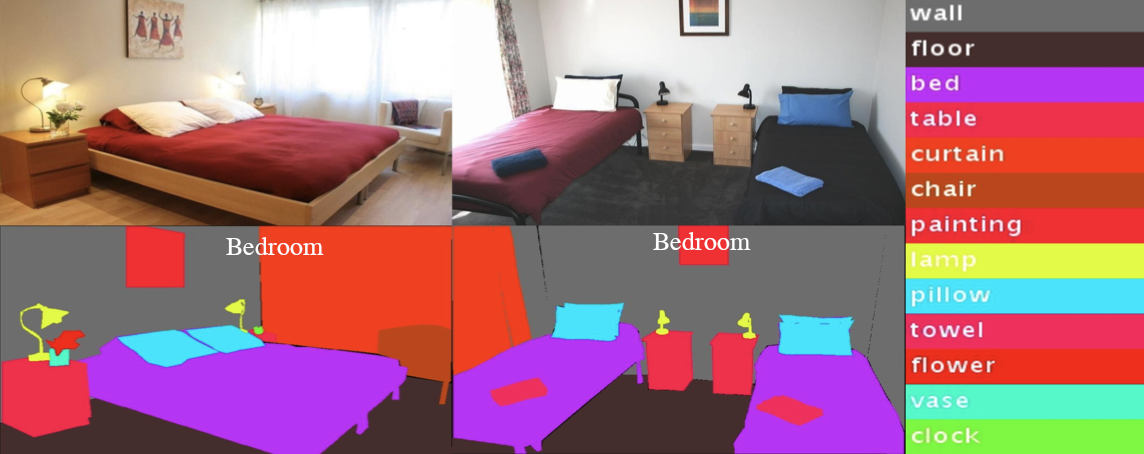
\includegraphics[height=0.5\textheight]{images/segment2.png}
        \caption{\cite{zhang2018context}.}
    \end{figure}
\end{frame}
\begin{frame}{Motywacje pracy}
    \begin{itemize}
        \item Nawigacja robota
        \begin{itemize}
            \item wykrywanie przeszkód
            \item zmiana zachowania pod wpływem znajdującego się pomieszczenia
        \end{itemize}
        \item Przewodnik dla osób niewidomych
        %  \item Poprawa działania całokształtu poprzez głębsze zrozuemienie otoczenia
    \end{itemize}
\end{frame}

\begin{frame}{Zbiór danych}
    \begin{figure}
        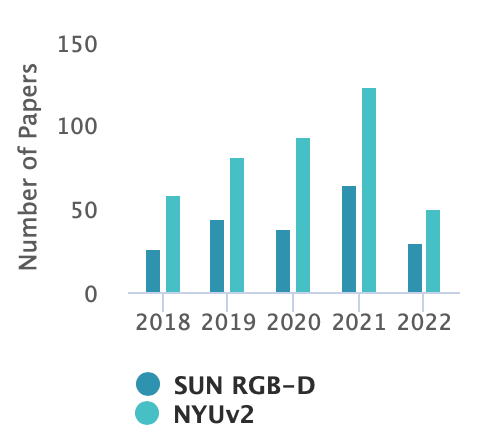
\includegraphics[height=0.7\textheight]{images/stats-dataset.png}
        \caption[]{Szacowana liczba cytowań w latach 2018-2022 \href{https://paperswithcode.com/dataset/sun-rgb-d}{[paperswithcode.com]}}
    \end{figure}
\end{frame}

\begin{frame}{Zbiór danych}
    \begin{columns}
        \begin{column}{0.5\textwidth}
            \begin{figure}
                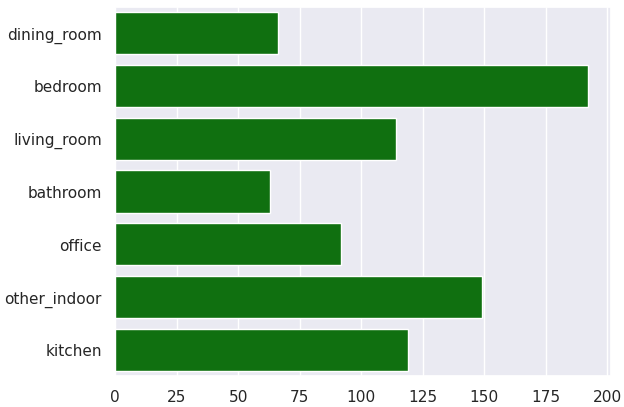
\includegraphics[width=\textwidth]{images/scene.png}
                \caption[]{Szacowana liczba cytowań w latach 2018-2022 \href{https://paperswithcode.com/dataset/sun-rgb-d}{[paperswithcode.com]}}
            \end{figure}
            
        \end{column}

        \begin{column}{0.5\textwidth}
            
            \begin{figure}
                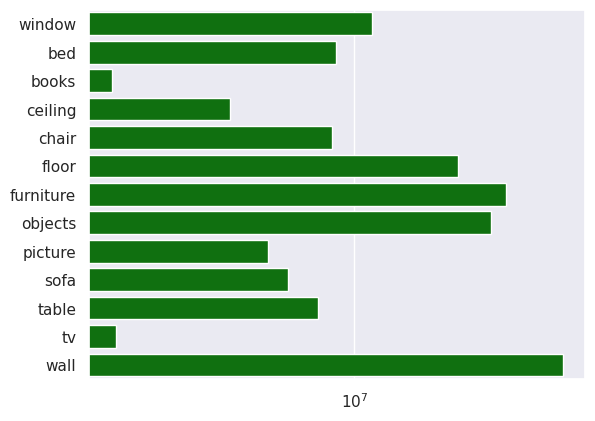
\includegraphics[width=\textwidth]{images/eda-seg13.png}
                \caption[]{Szacowana liczba cytowań w latach 2018-2022 \href{https://paperswithcode.com/dataset/sun-rgb-d}{[paperswithcode.com]}}
            \end{figure}
        \end{column}
    \end{columns}
\end{frame}
\section*{Rozwiązanie problemu}
\begin{frame}{Rozwiązanie problemu - przedstawienie architektury}
    \begin{figure}
        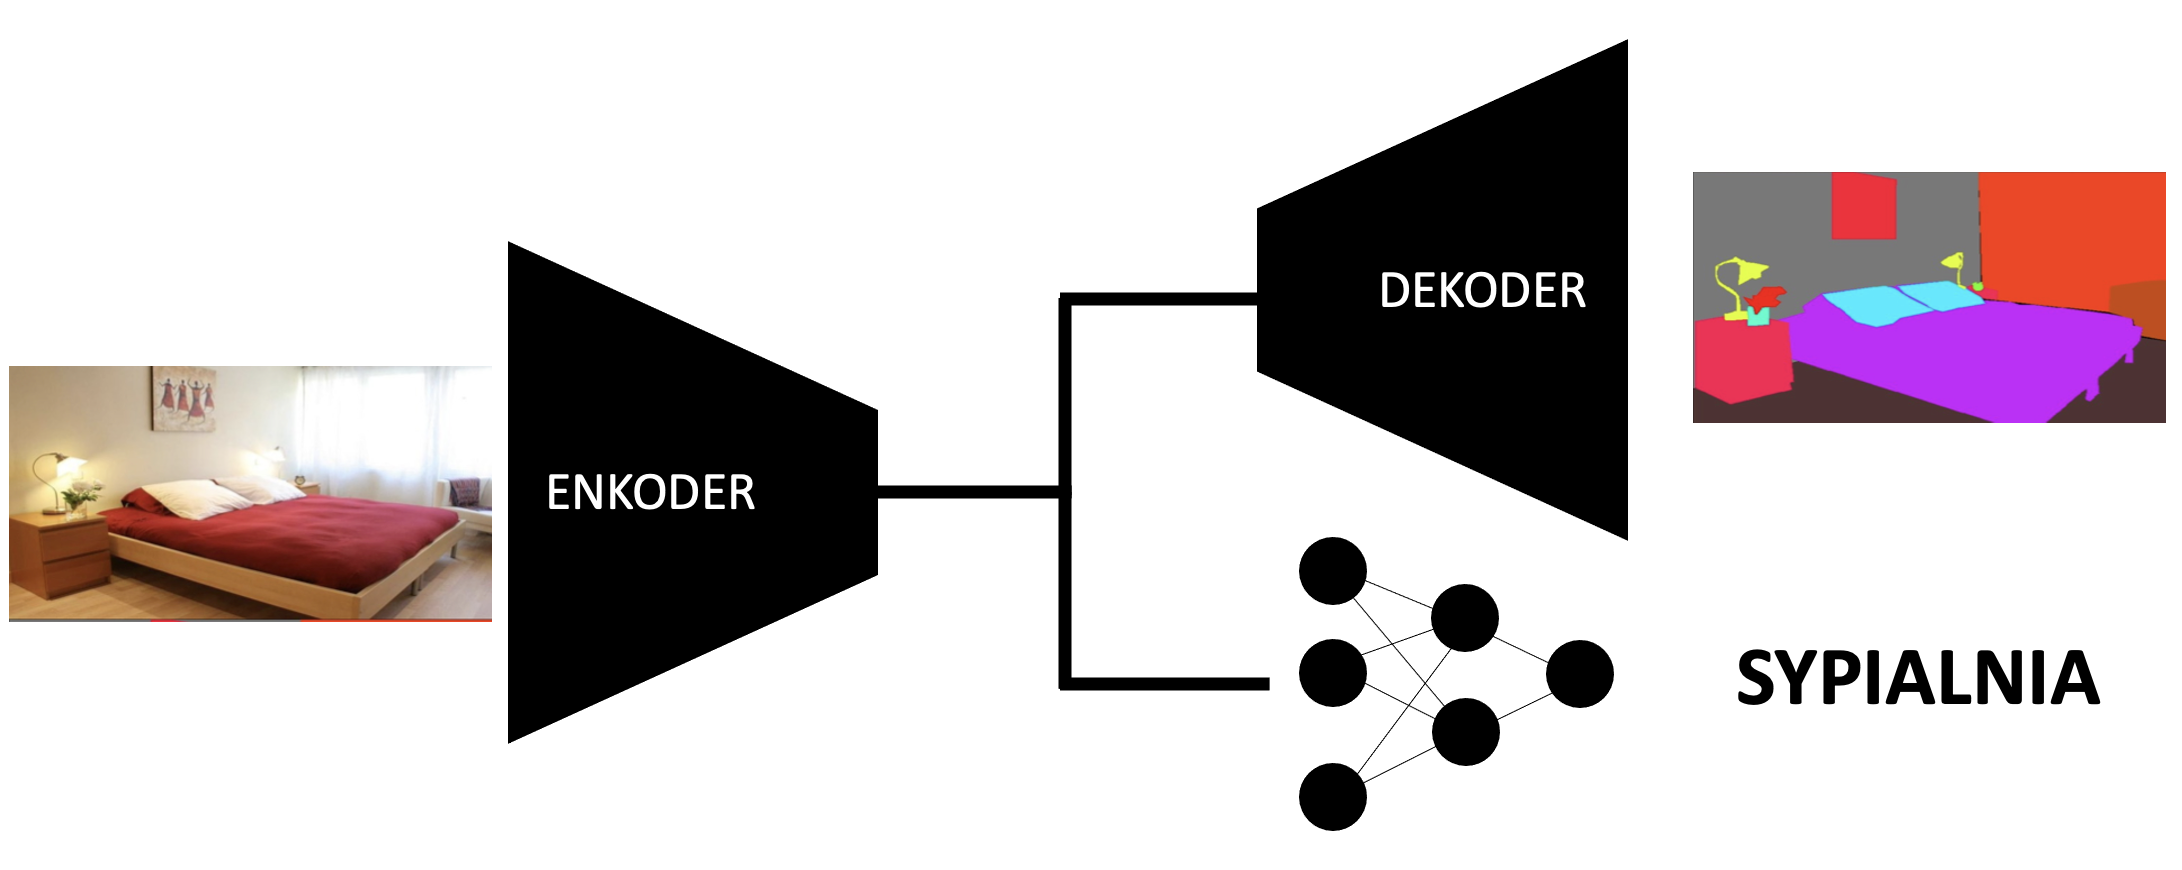
\includegraphics[width=\textwidth]{images/cep_arch.png}
        \caption{Architektura sieci zastosowana w pracy inżynierskiej.}
    \end{figure}
\end{frame}
\section*{Podejście jednozadaniowe}
\begin{frame}{Rozwiązanie problemu}
    \begin{columns}
        \begin{column}{0.5\textwidth}
            \begin{figure}
                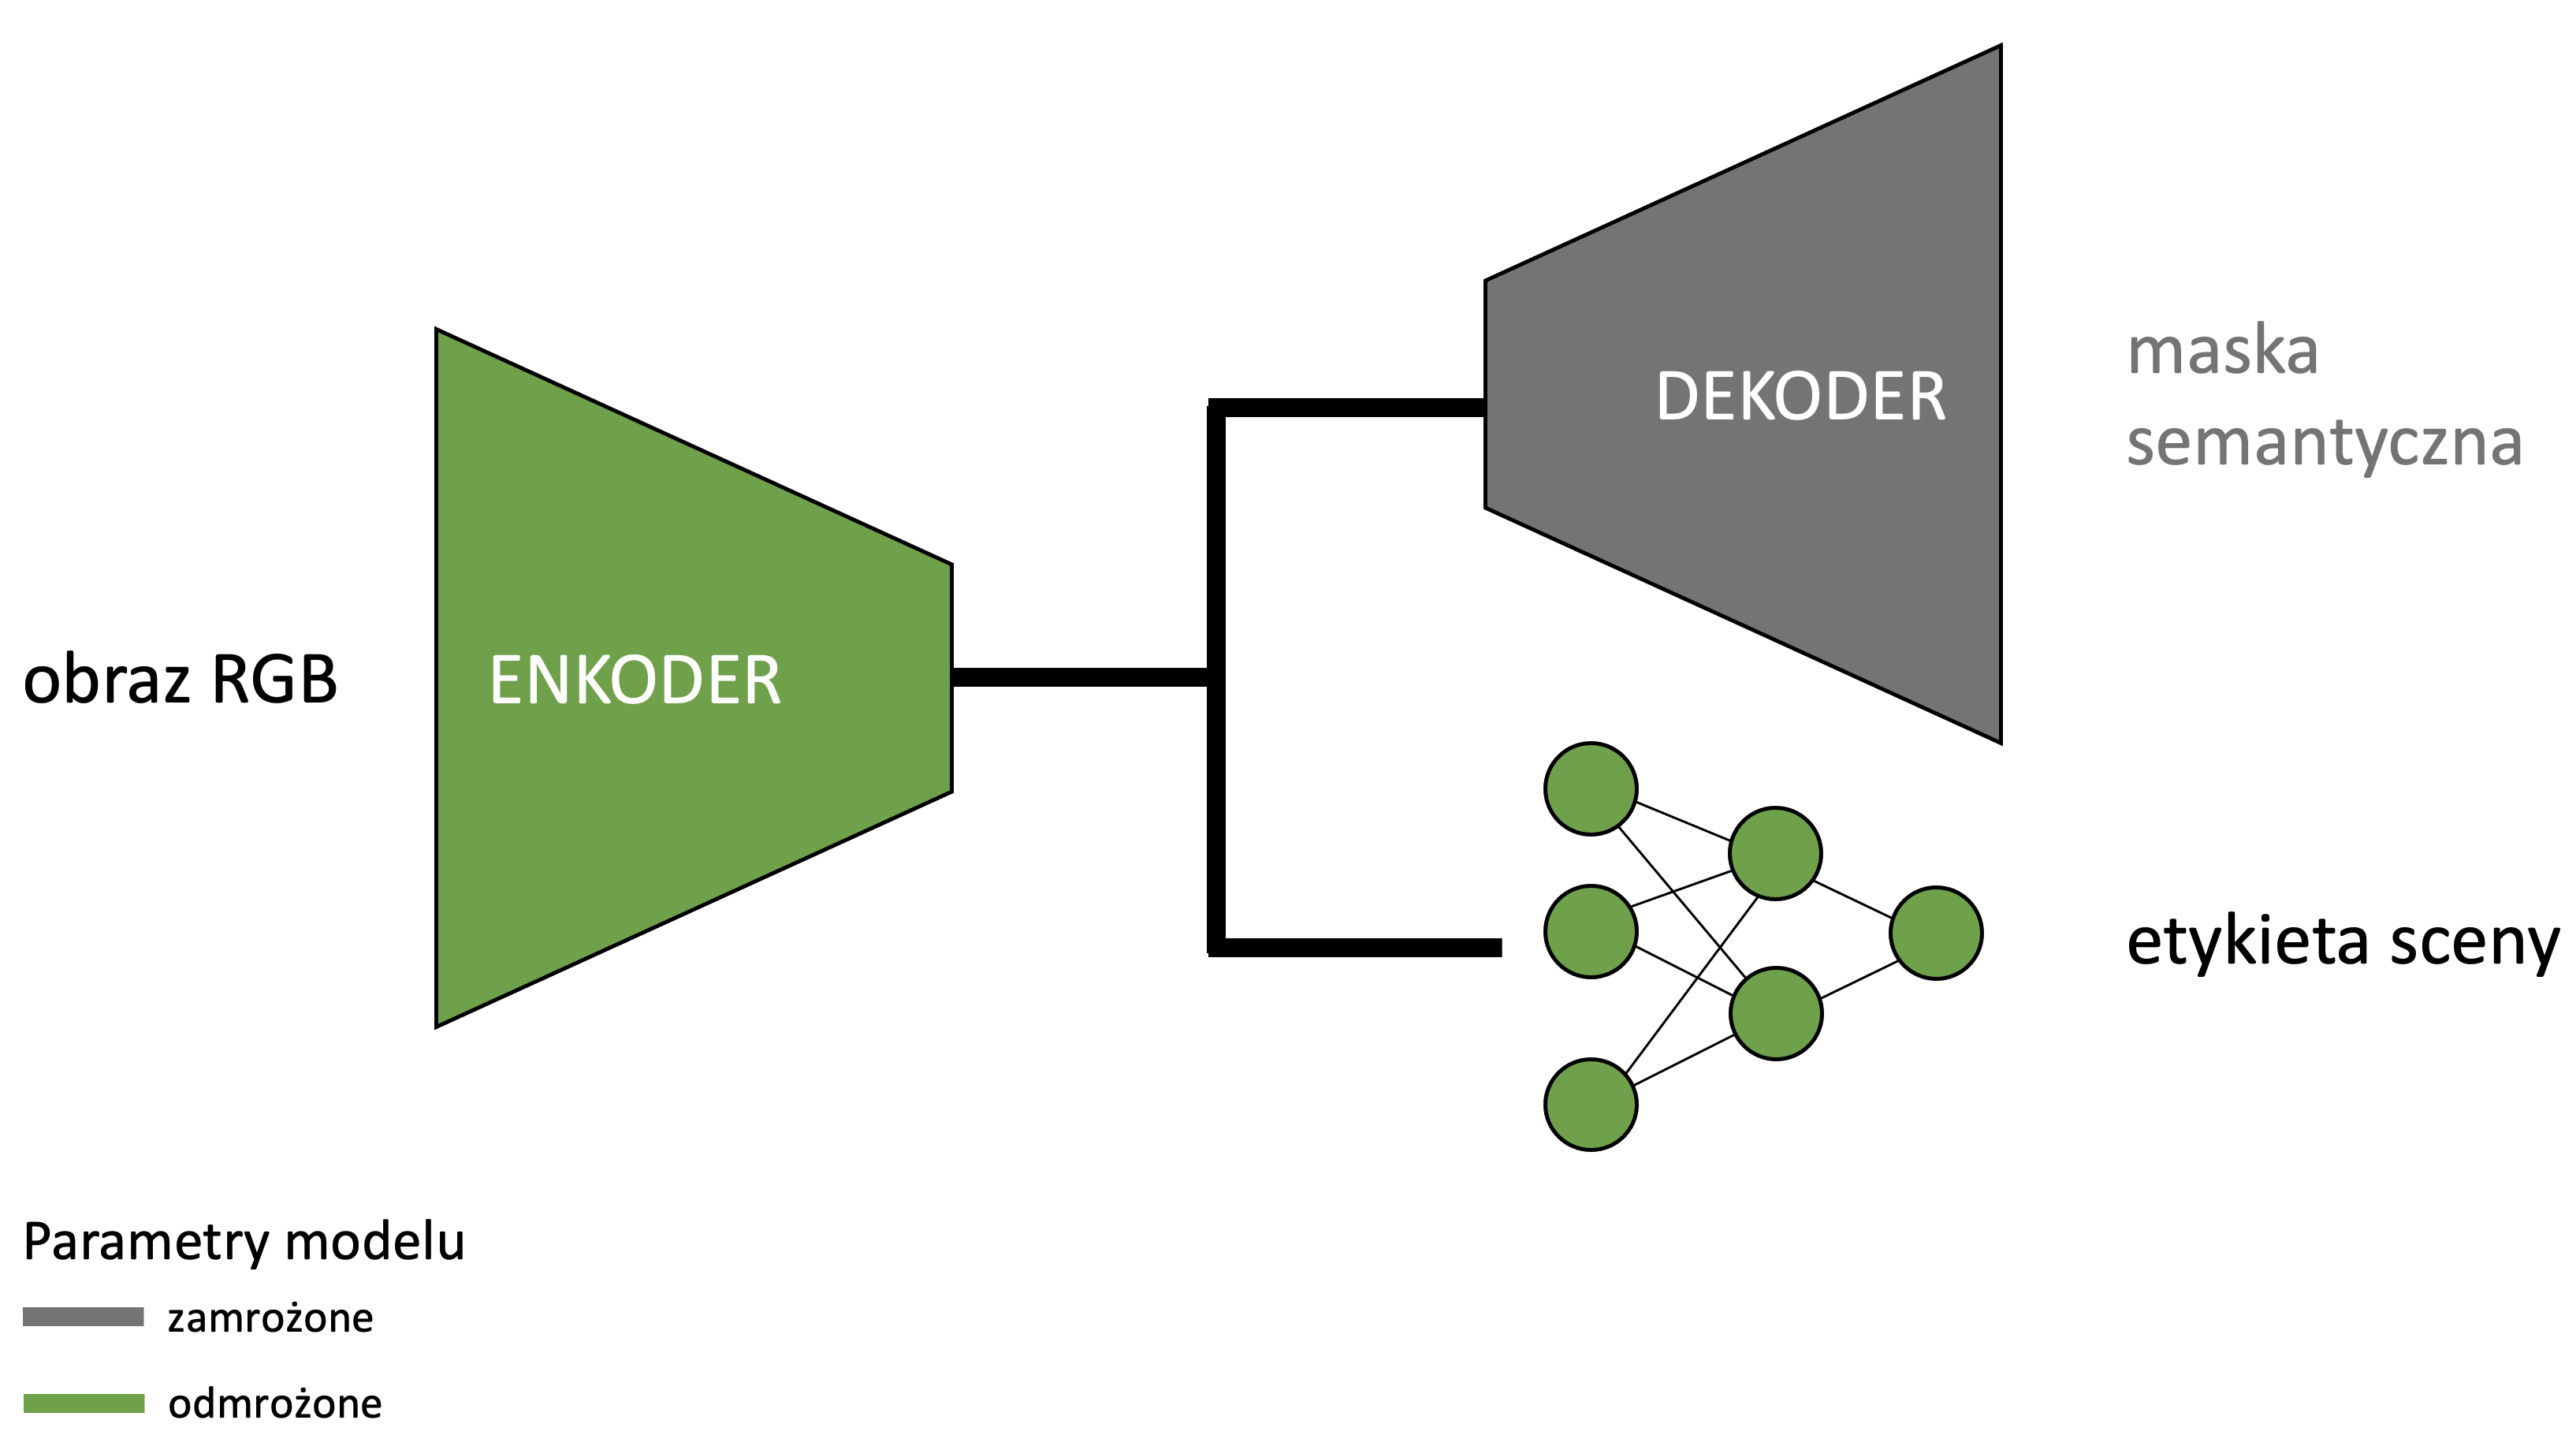
\includegraphics[width=\textwidth]{images/arch:scene.png}
                \caption{Architektura sieci wyłącznie w zadaniu klasyfikacji.}
            \end{figure}
            
        \end{column}
        
        \begin{column}{0.5\textwidth}
            \begin{figure}
                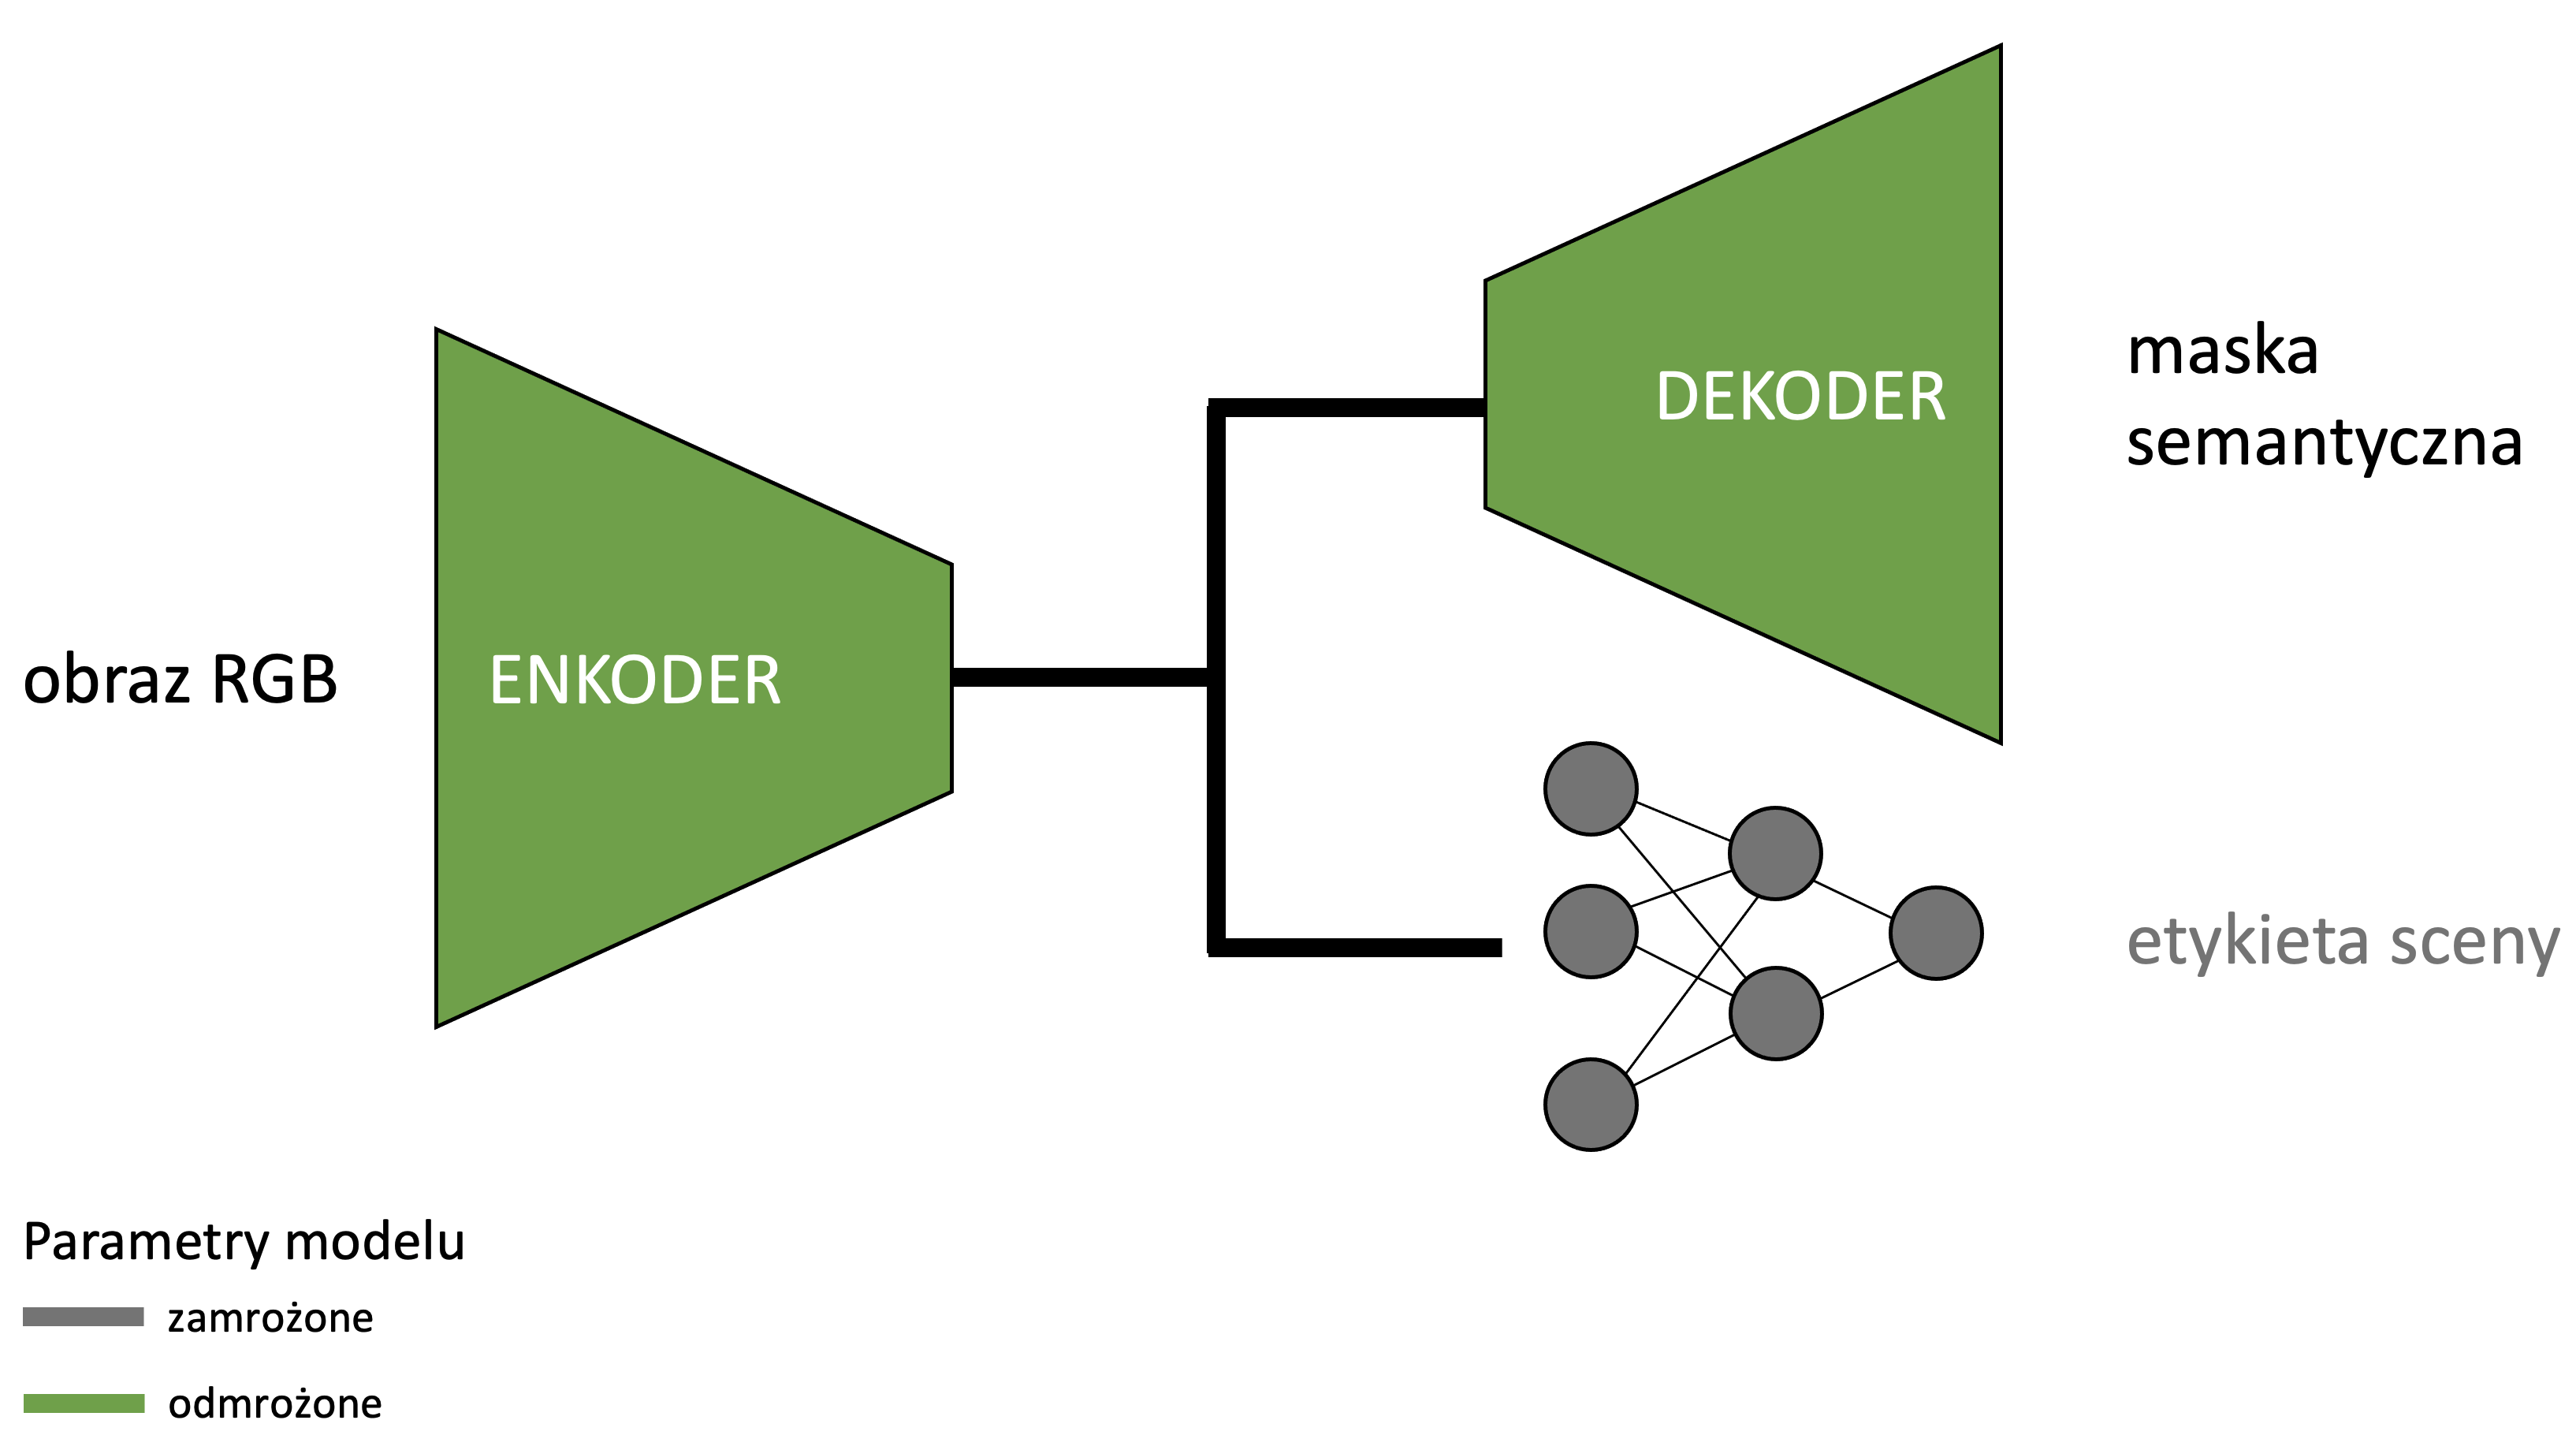
\includegraphics[width=\textwidth]{images/arch:seg.png}
                \caption{Architektura sieci wyłącznie w zadaniu segmentacji semantycznej.}
            \end{figure}
            
        \end{column}
    \end{columns}

\end{frame}
% \begin{frame}{Rozwiązanie problemu - segmentacja}
%     \begin{figure}
%         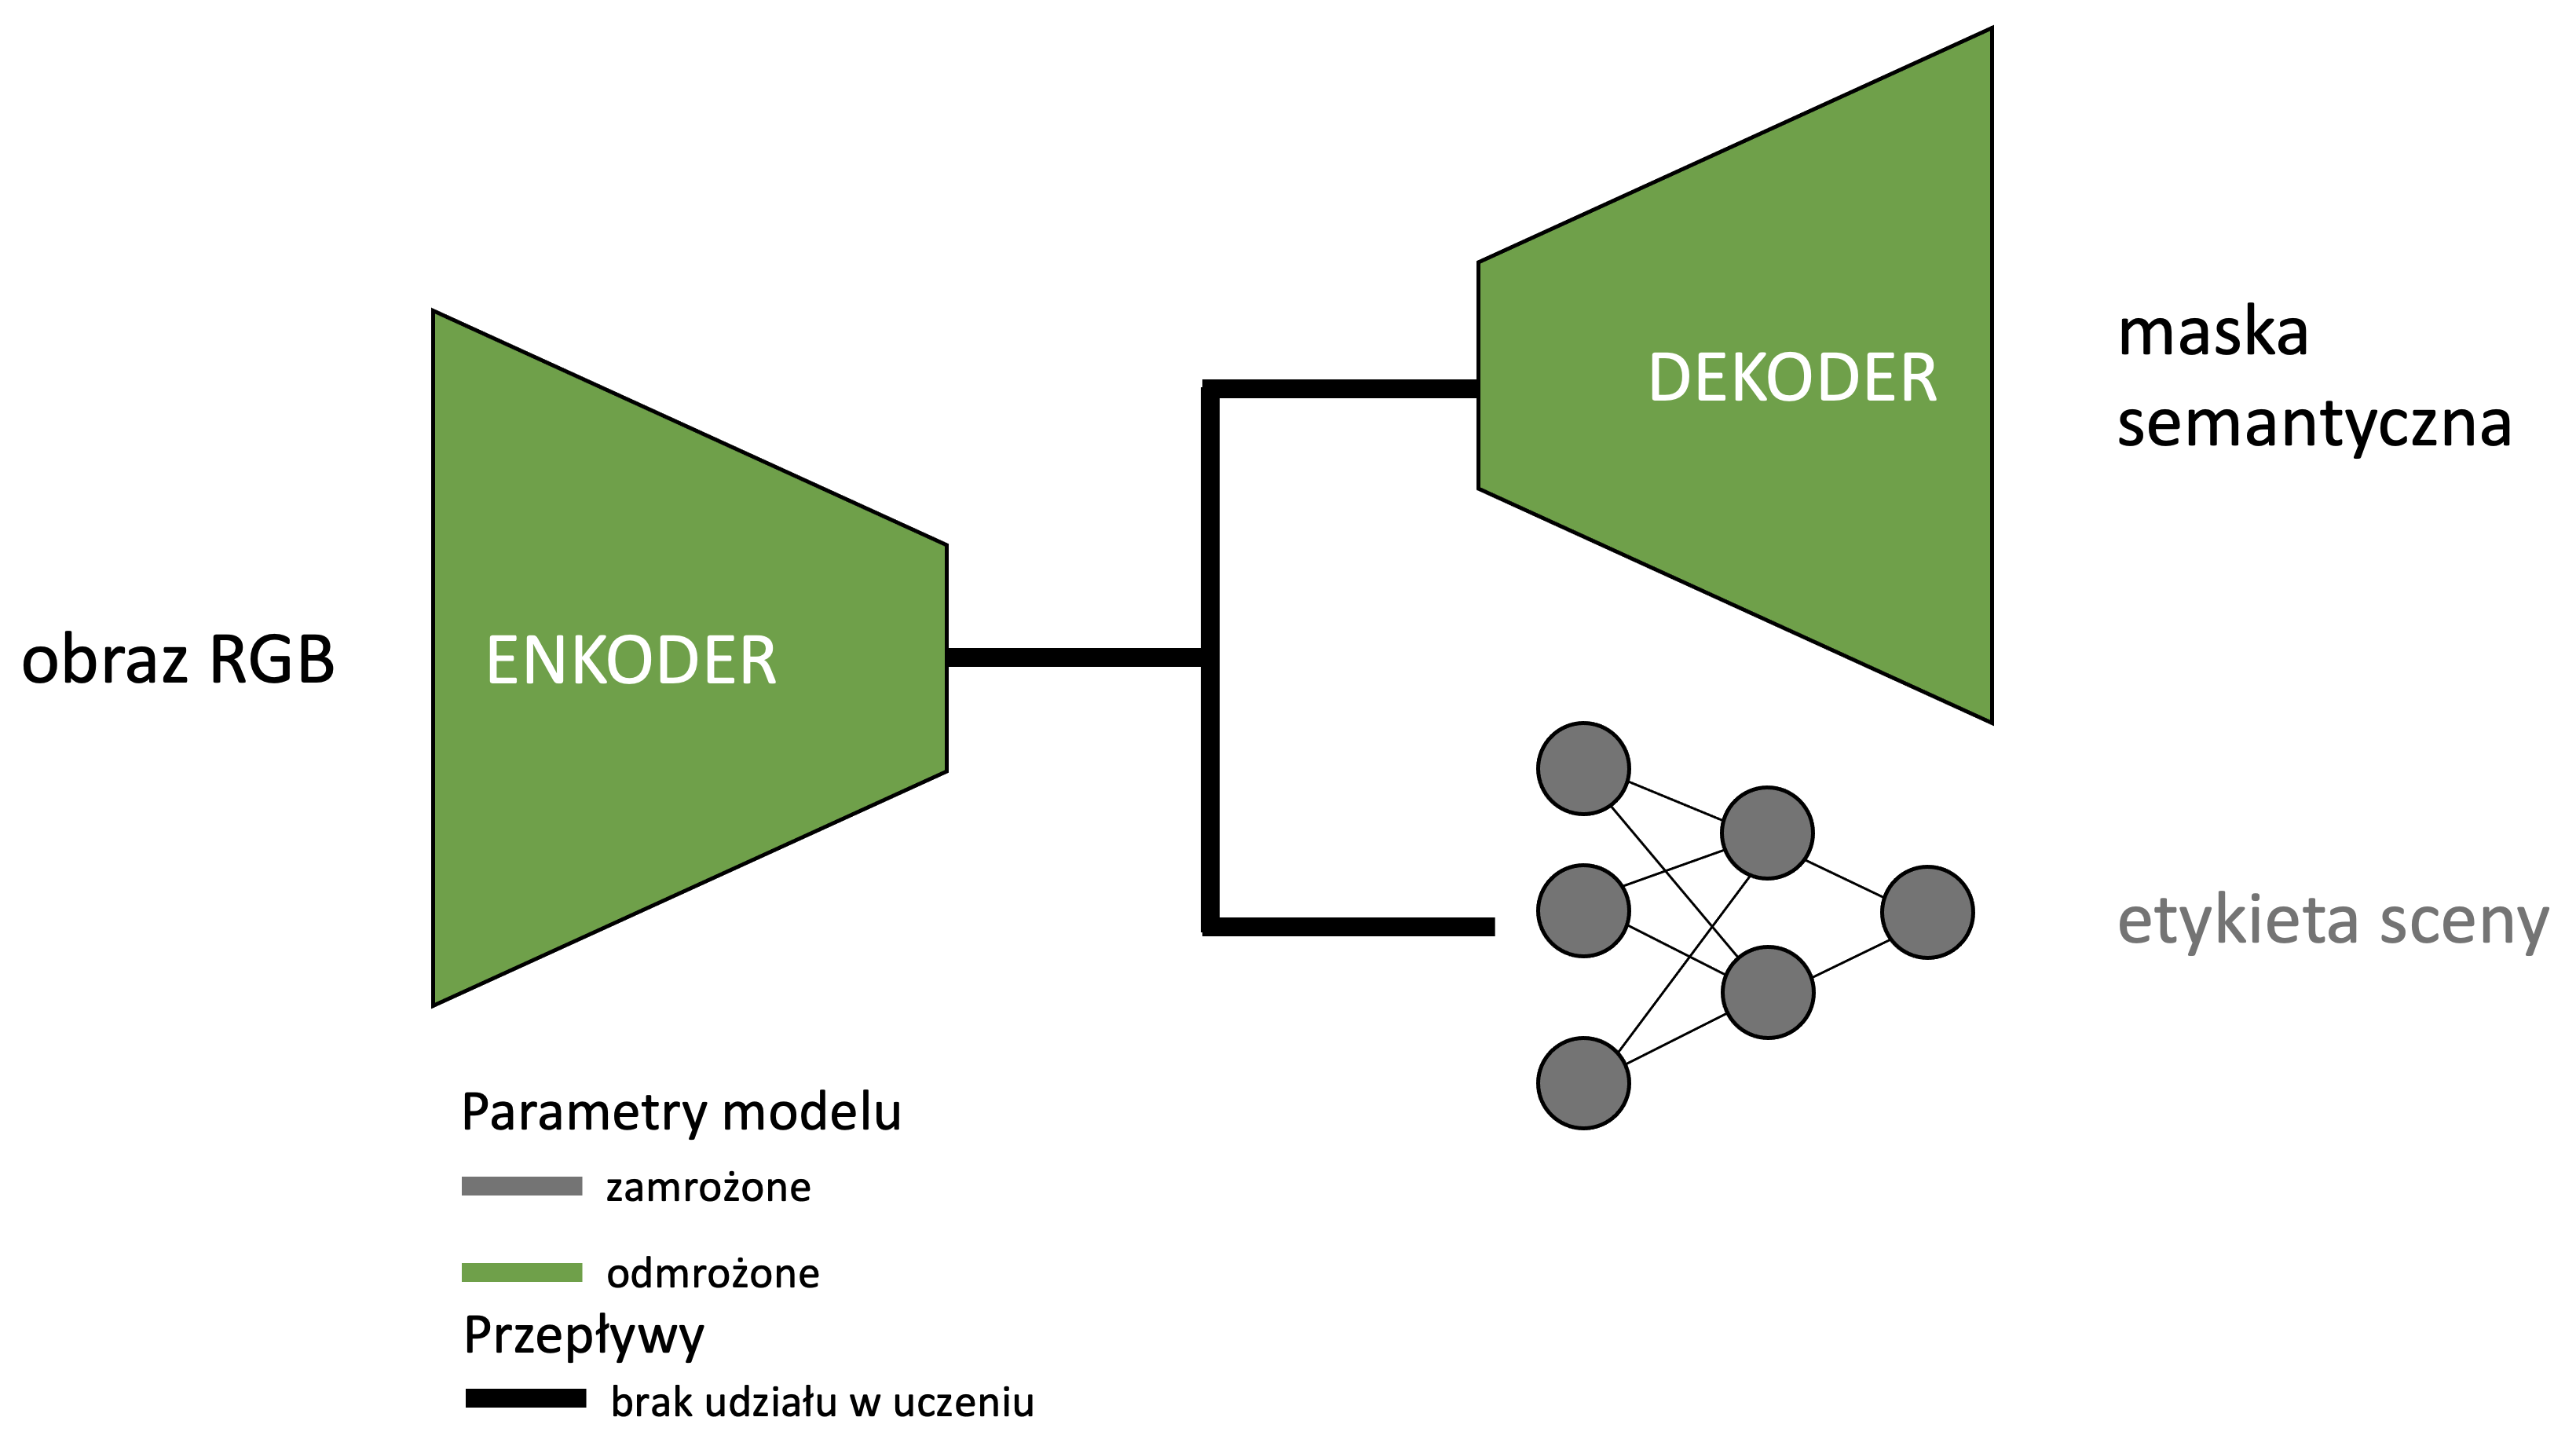
\includegraphics[width=\textwidth]{images/fc-freezed.png}
%         \caption{Architektura sieci wyłącznie w zadaniu segmentacji semantycznej.}
%     \end{figure}
% \end{frame}
\section*{Podejście wielozadaniowe}
\begin{frame}{Rozwiązanie problemu}
    \begin{figure}
        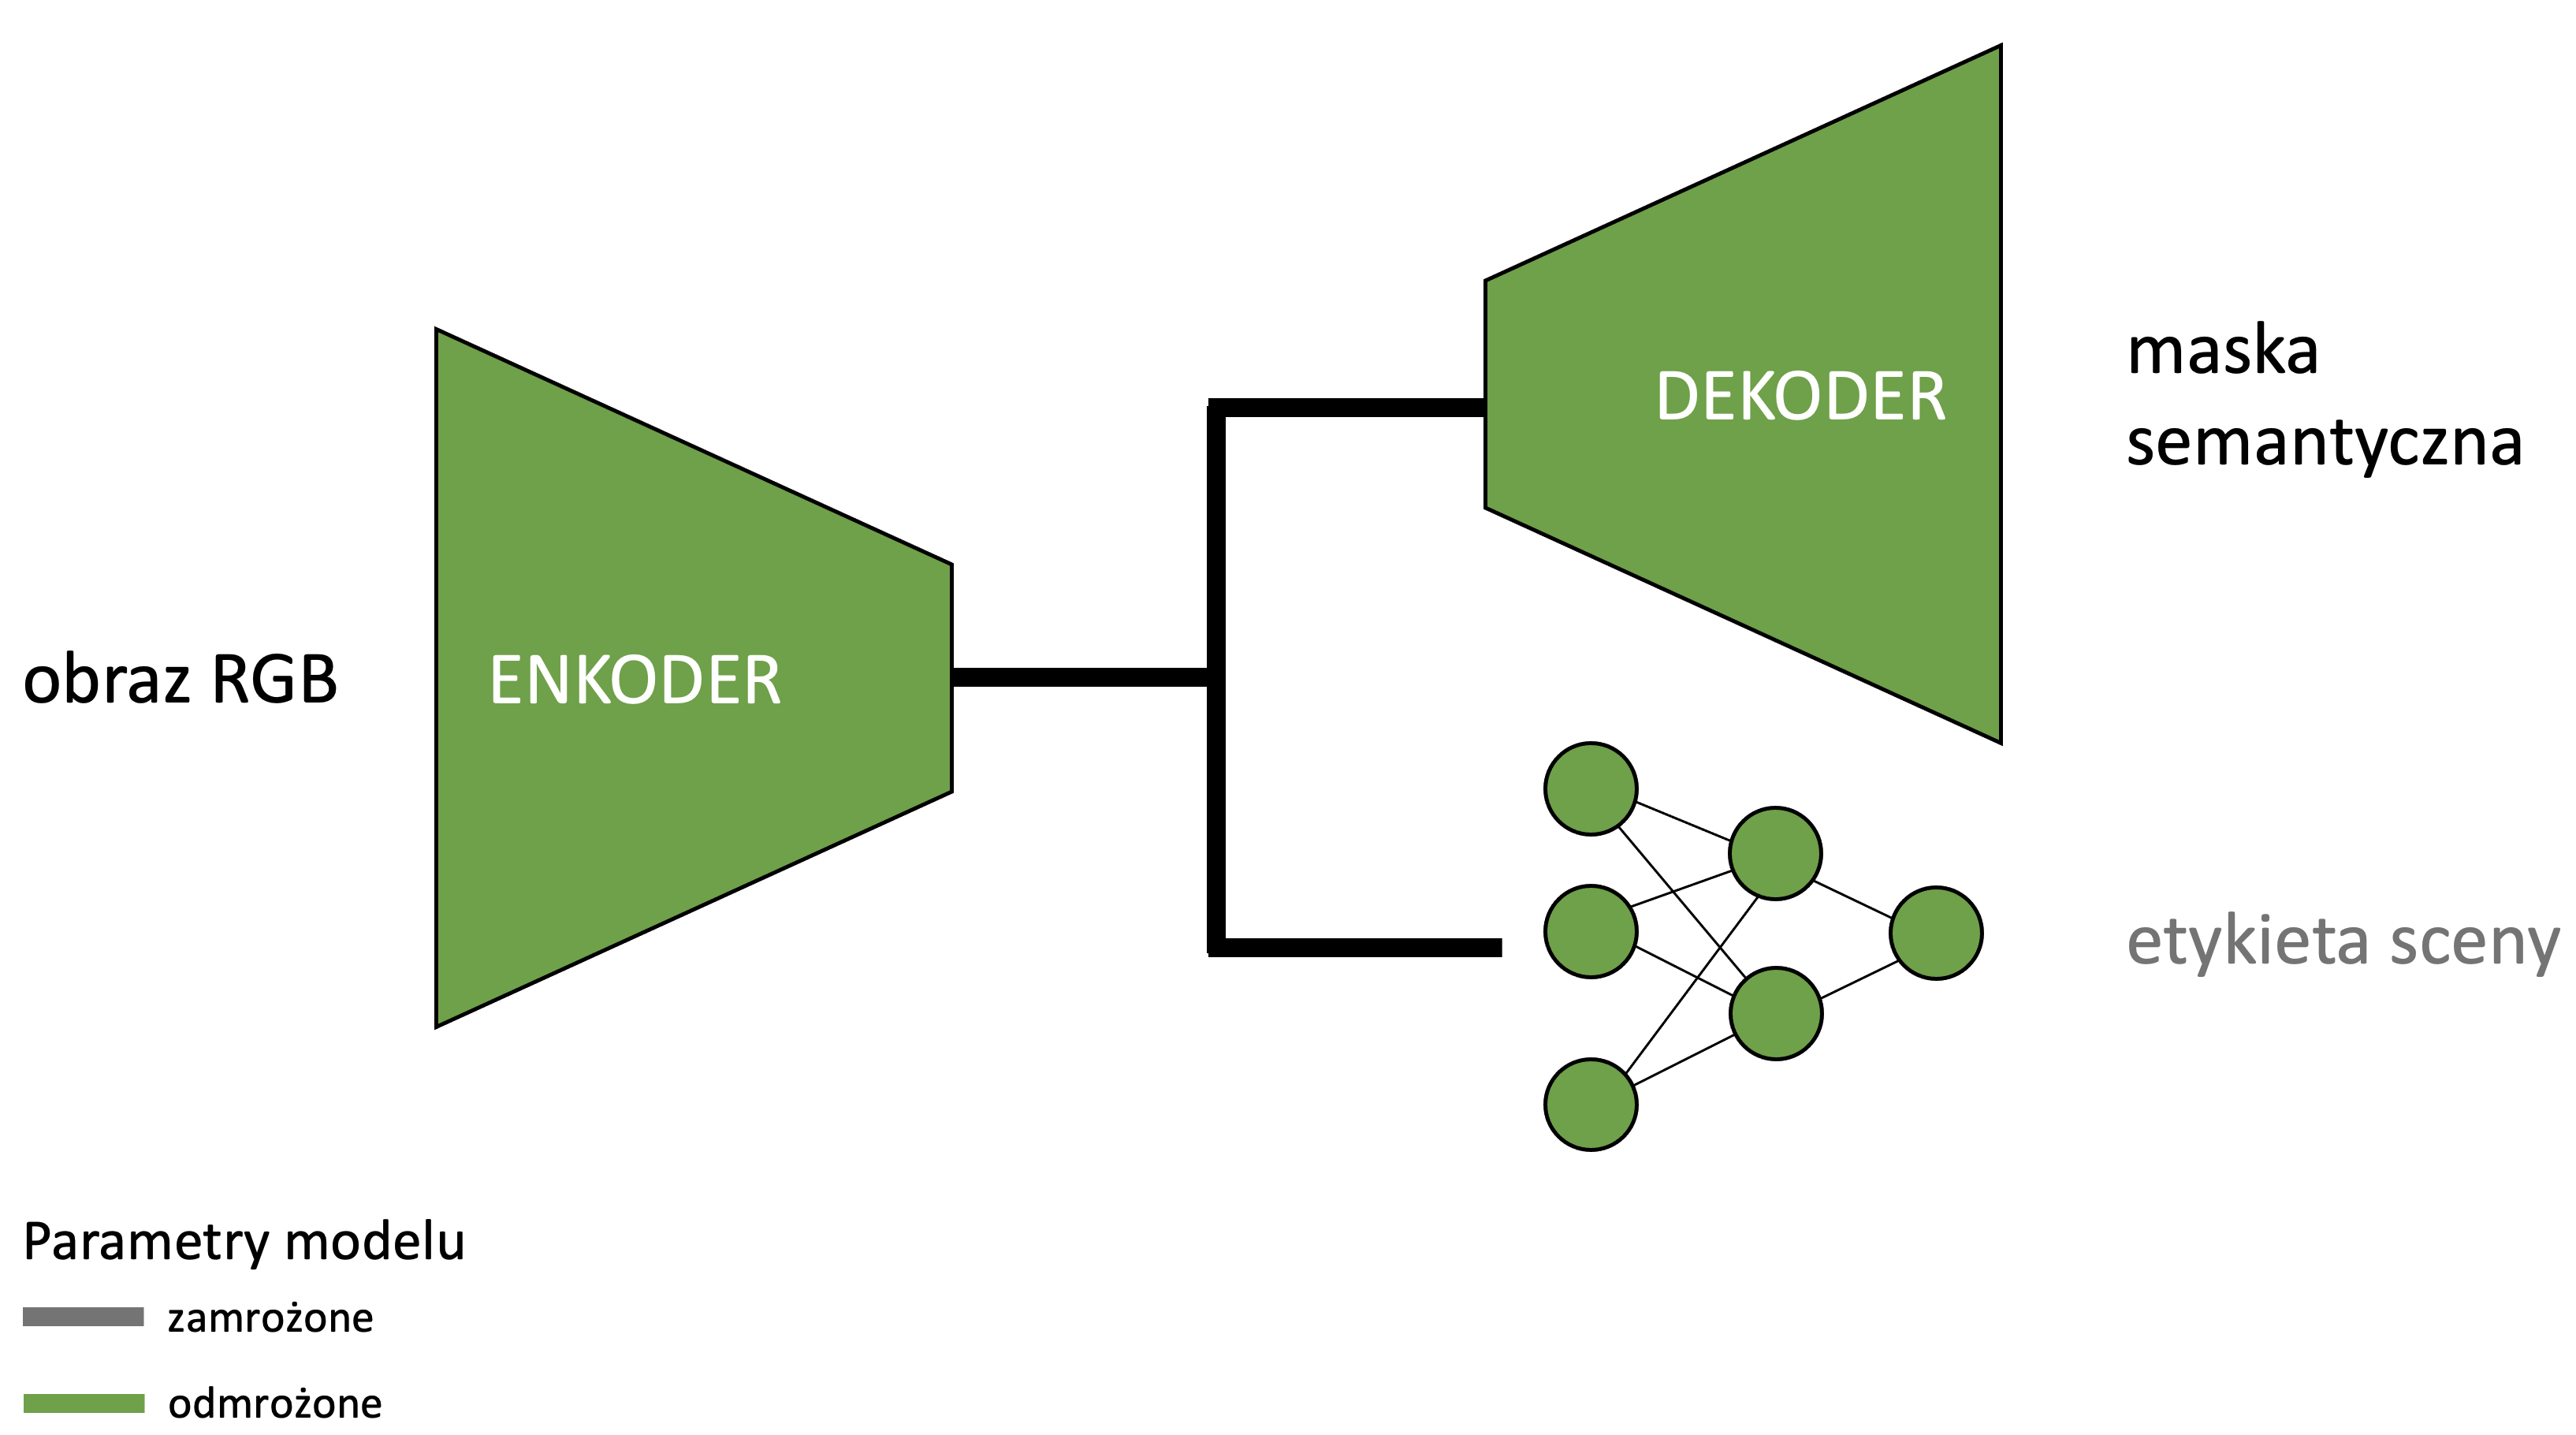
\includegraphics[width=\textwidth]{images/arch:full.png}
        \caption{Architektura sieci jako uczenie wielozadaniowego.}
    \end{figure}
\end{frame}
    
\begin{frame}{Wyniki - klasyfikacja}
    \begin{figure}
        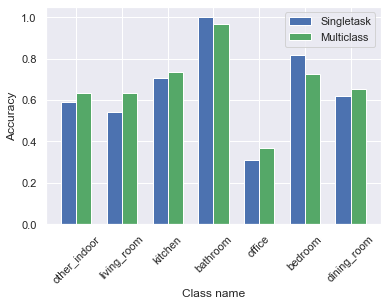
\includegraphics[width=0.75\textwidth]{images/scene_comp.png}
        \caption{Porównanie dokładności dla każdej z klas w zadaniu klasyfikacji pomieszczeń}
    \end{figure}
\end{frame}    
    
\begin{frame}{Wyniki - segmentacja}
    \begin{figure}
        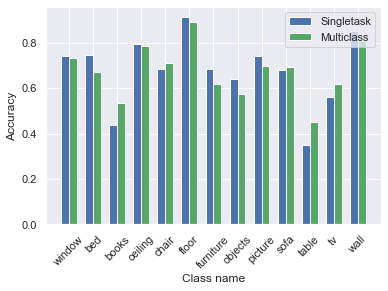
\includegraphics[width=0.75\textwidth]{images/seg_comp.png}
        \caption{Porównanie dokładności dla każdej z klas w zadaniu segmentacji semantycznej}
    \end{figure}
\end{frame}    
 
    
% \begin{frame}{Wyniki pracy - próba kontrolna}
        
%     \begin{figure}
%         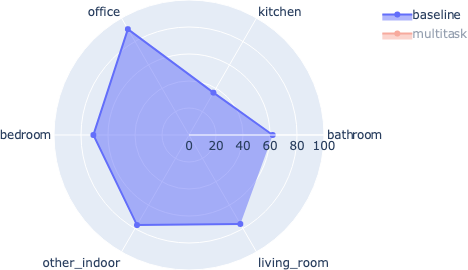
\includegraphics[width=\textwidth]{images/classification_polar_baseline.png}
%         \caption{IoU\% dla każdej etykiety w zadaniu klasyfikacji.}
%     \end{figure}
% \end{frame}
% \begin{frame}{Wyniki pracy - próba badawcza}
%     \begin{figure}
%         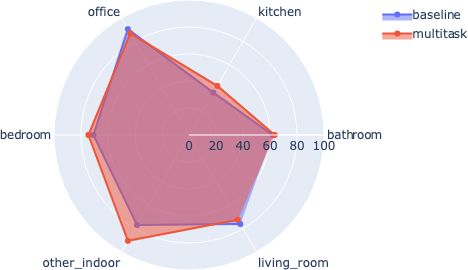
\includegraphics[width=\textwidth]{images/classification_polar.png}
%         \caption{Porównanie IoU\% dla każdej z etykiet w zadaniu klasyfikacji}
%     \end{figure}
% \end{frame}


% \begin{frame}{Wyniki pracy - próba kontrolna}
        
%     \begin{figure}
%         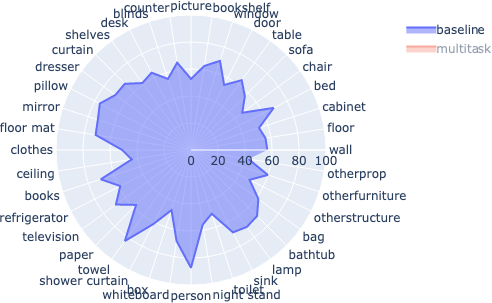
\includegraphics[width=\textwidth]{images/segmentation_polar_baseline.png}
%         \caption{IoU\% dla każdej etykiety w zadaniu segmentacji.}
%     \end{figure}
% \end{frame}
% \begin{frame}{Wyniki pracy - próba badawcza}
%     \begin{figure}
%         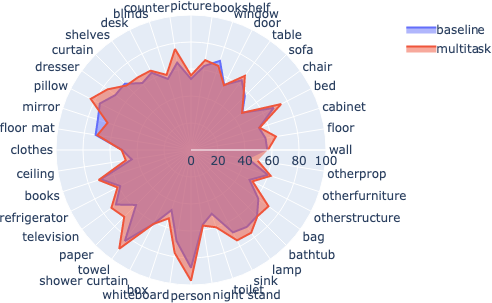
\includegraphics[width=\textwidth]{images/segmentation_polar.png}
%         \caption{Porównanie IoU\% dla każdej z etykiet w zadaniu segmentacji.}
%     \end{figure}
% \end{frame}


\begin{frame}{Wnioski}
    Ucznie wielozadaniowe pomaga osiągnać lepsze wyniki.
    \begin{table}[]
        \begin{tabular}{c|cc}
        zadanie/{[}\%{]} & Acc jednozadaniowe & Acc wielozadaniowe \\ \hline
        segmentacja      & 67.87               & 67.48  \footnotesize{\textbf{$-$0.39}}        \\
        klasyfikacja     & 65.50               & 67.45  \footnotesize{\textbf{+1.95}}        \\ \hline
        średnia          & 66.69               & 67.47  \footnotesize{\textbf{+0.78}}       
        \end{tabular}
        \end{table}
    
\end{frame}
\begin{frame}{Podsumowanie}
    \begin{itemize}
        \item Cele pracy - klasyfikacja sceny i segmentacja semantyczna zostały spełnione
        \item Średnia dokładności została zwiększona poprzez uczenie wielozadaniowe
        \item Wielkość modelu zmniejszyła się prawie dwukrotnie, co bezpośrednio wpływa na czas inferencji
        \item Dalsze możliwości rozwoju:
        \begin{itemize}
            \item inferencja na robocie Tiago
            \item sprawdzenie czasu inferencji
        \end{itemize}
    \end{itemize}

    

\end{frame}
\begin{frame}[plain, allowframebreaks,noframenumbering]{Bibliografia}
    
    \bibliography{presentation}
    \bibliographystyle{abbrv}
    
\end{frame}
\end{document}





%     \begin{frame}{Agenda}
%         \setbeamertemplate{section in toc}[sections numbered]
%         \tableofcontents%[hideallsubsections]
%     \end{frame}
%     \section[Cel pracy]{Cel pracy}
%         \begin{frame}{Cel}
%             % \begin{itemize}
%             %     \item Zrozumienie środowiska wewnątrz budynku
%             %     \item Klasyfikacja pomieszczeń
%             % \end{itemize}

%             Przygotowanie systemu, który otrzymując obraz przedstawiający środowisko domowe będzie informował o znajdujących się tam przedmiotach oraz równocześnie klasyfikował pomieszczenie
%         \end{frame}
%     % ########################################################################################################
%     \section[Wprowadzenie do tematyki pracy]{Wprowadzenie do tematyki pracy}

%     \begin{frame}{Klasyfikacja sceny}
%         \begin{figure}
%             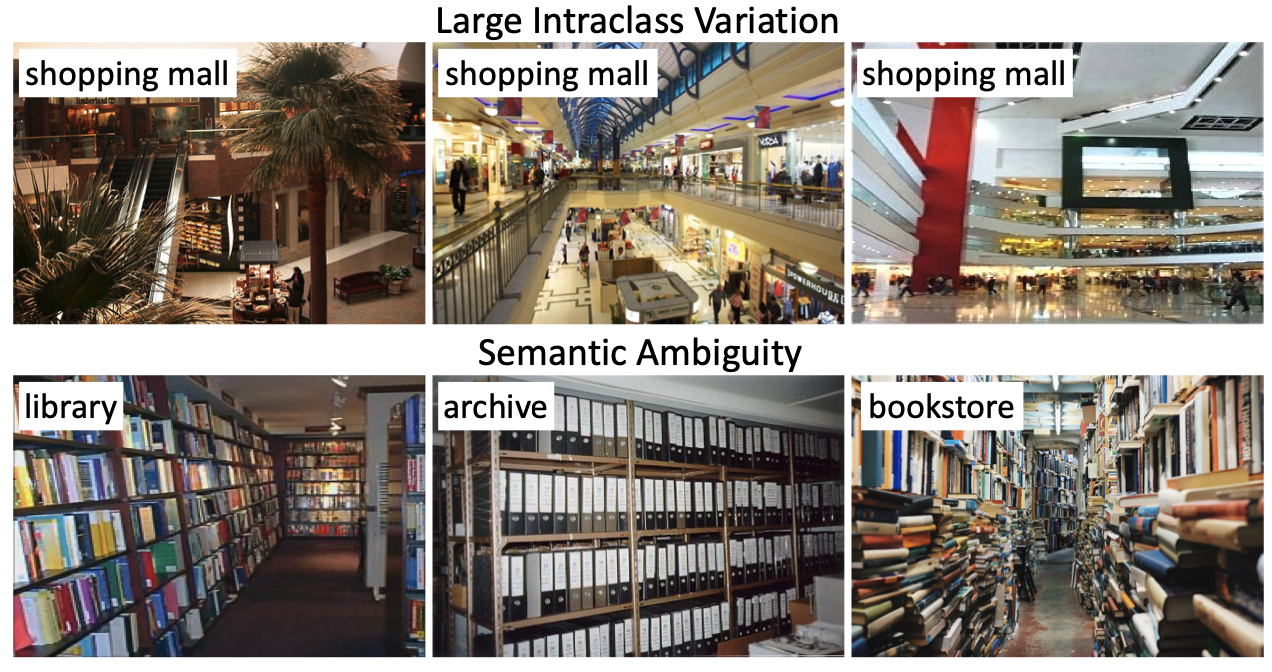
\includegraphics[width=\textwidth]{images/scene_class.png}
%             \caption{Problem różrnorodności wewnątrzklasowej oraz wieloznaczności semantycznej \cite{zeng2021deep}.}
%         \end{figure}
        
%     \end{frame}

%     \begin{frame}{Splotowa sieć klasyfikacyjna}
%         \begin{figure}
%             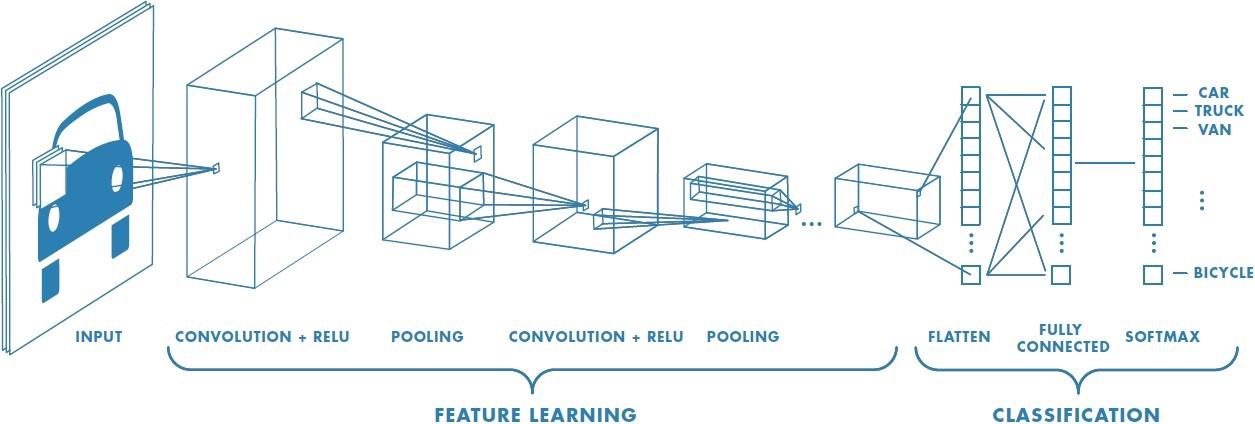
\includegraphics[width=\textwidth]{images/classification.jpeg}
%             \caption{https://towardsdatascience.com/a-comprehensive-guide-to-convolutional-neural-networks-the-eli5-way-3bd2b1164a53}
%         \end{figure}
        
%     \end{frame}

%     \begin{frame}{Autoenkoder}
%         \begin{figure}
%             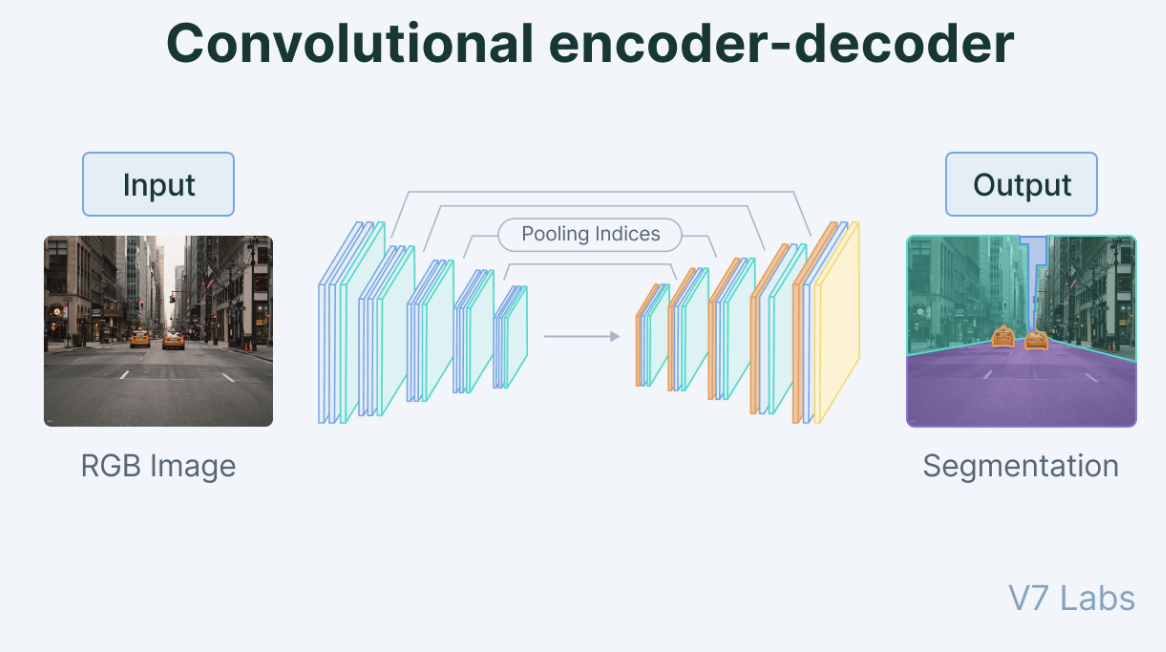
\includegraphics[width=\textwidth]{images/autoencoder.png}
%             \caption{https://www.v7labs.com/blog/autoencoders-guide}
%         \end{figure}
        
%     \end{frame}


%     \begin{frame}{Uczenie wielozadaniowe}
%         \begin{figure}
%             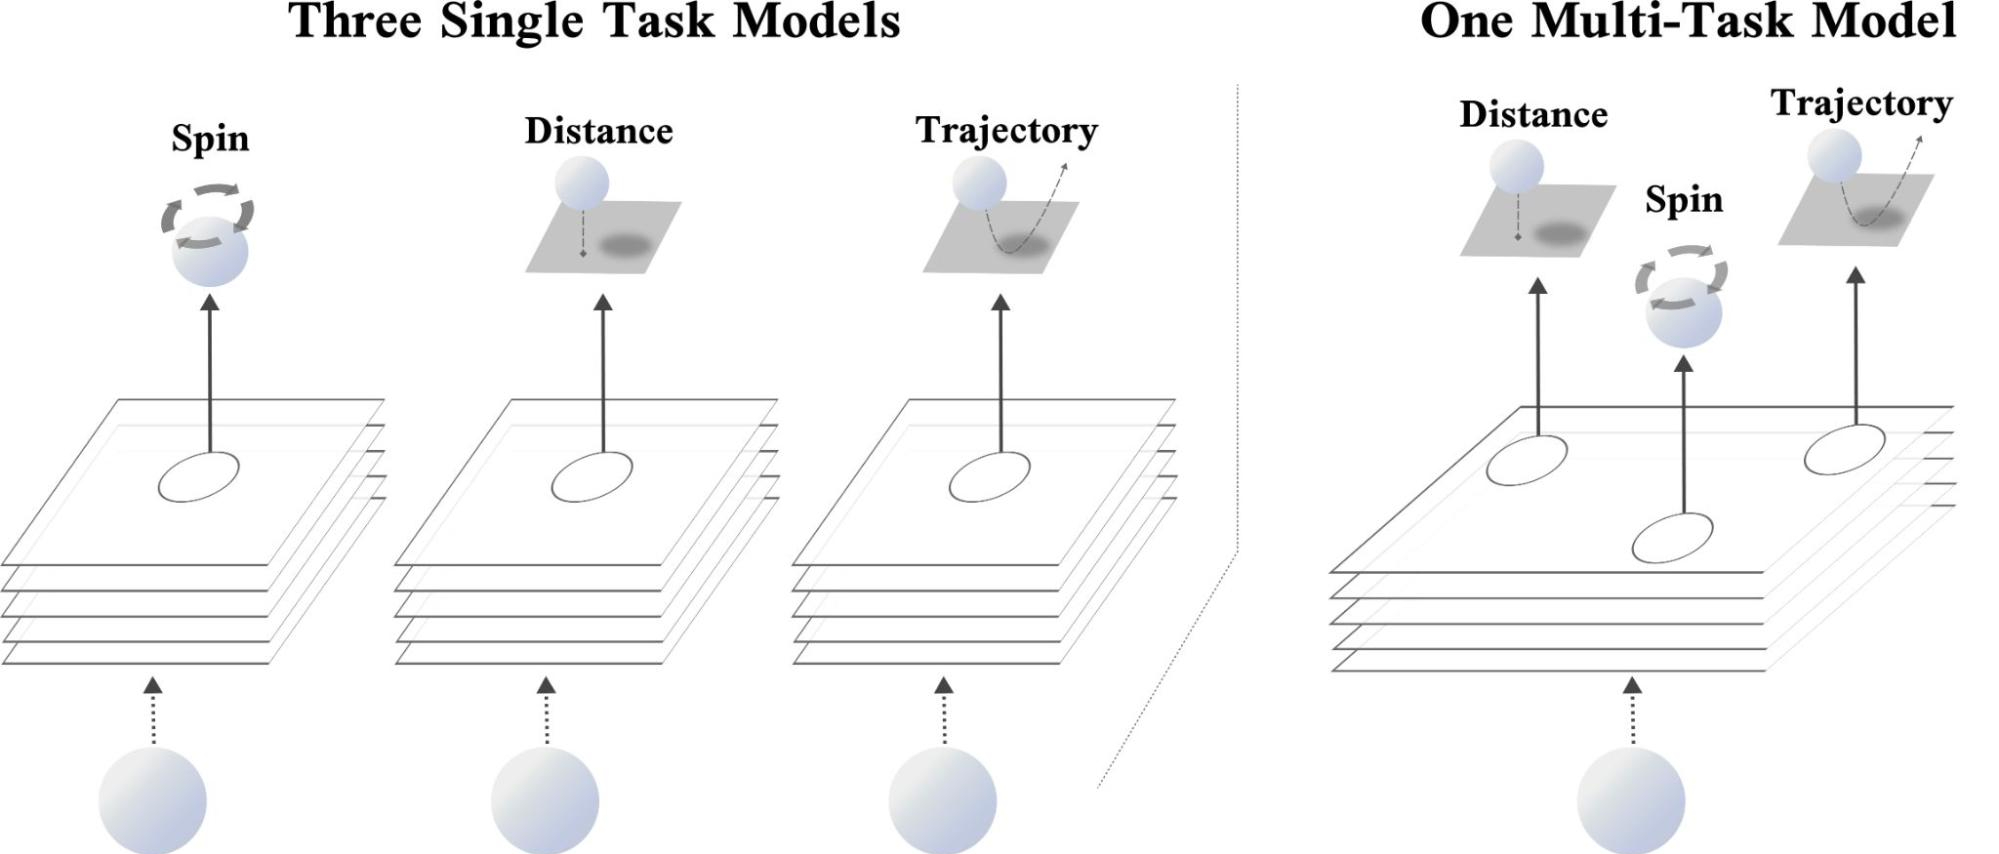
\includegraphics[width=\textwidth]{images/multitask.jpg}
%             \caption{https://ai.googleblog.com/2021/10/deciding-which-tasks-should-train.html}
%         \end{figure}
        
%     \end{frame}
%     % ########################################################################################################
%     % ########################################################################################################
%     \section[Przegląd rozwiązań]{Przegląd rozwiązań}
%     % ########################################################################################################
    
%     % ########################################################################################################
%     % \begin{frame}{Przegląd rozwiązań}
        
%         % \begin{figure}
%             %     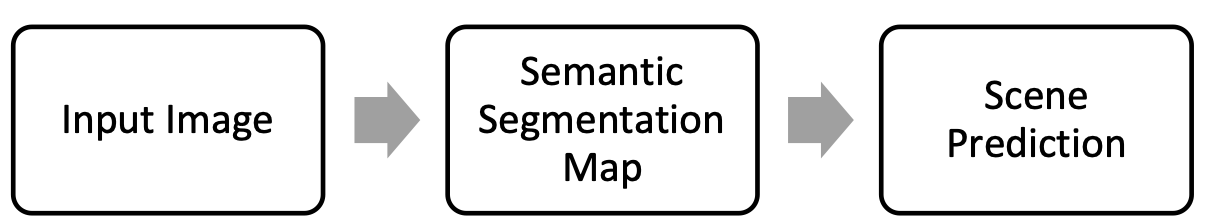
\includegraphics[width=\textwidth]{images/linear-seg-reg-pipeline.png}
%             %     \caption{Semantic segmentation as image representation for scene recognition 2014 \cite{bassiouny2014semantic}.}
%             % \end{figure}
%             % \end{frame}
            
%             % ########################################################################################################
%             % ########################################################################################################
%             \begin{frame}{Przegląd rozwiązań}
                
%                 \begin{figure}
%                     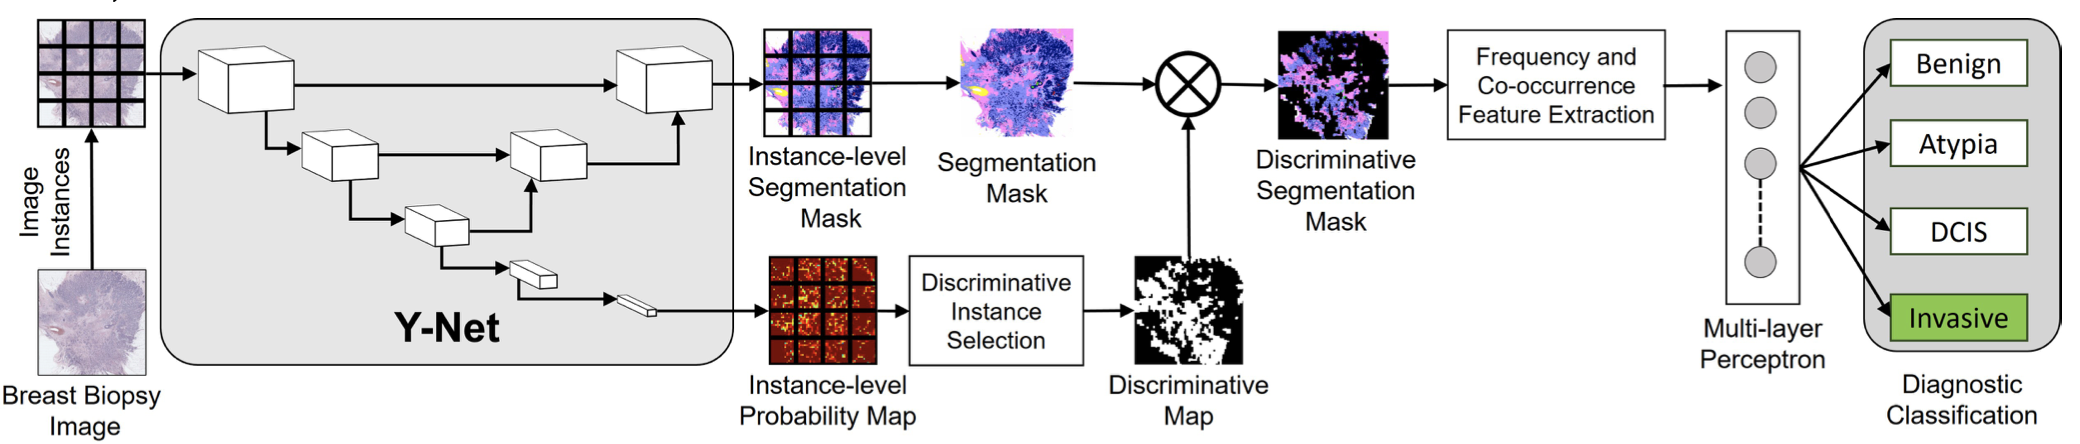
\includegraphics[width=\textwidth]{images/y-net.png}
%                     \caption{Y-Net: Joint Segmentation and Classification for Diagnosis of Breast Biopsy Images 2018 \cite{mehta2018net}.}
%                 \end{figure}
%             \end{frame}
            
%             % ########################################################################################################
%             \begin{frame}{Przegląd rozwiązań}
                
%                 \begin{figure}
%                     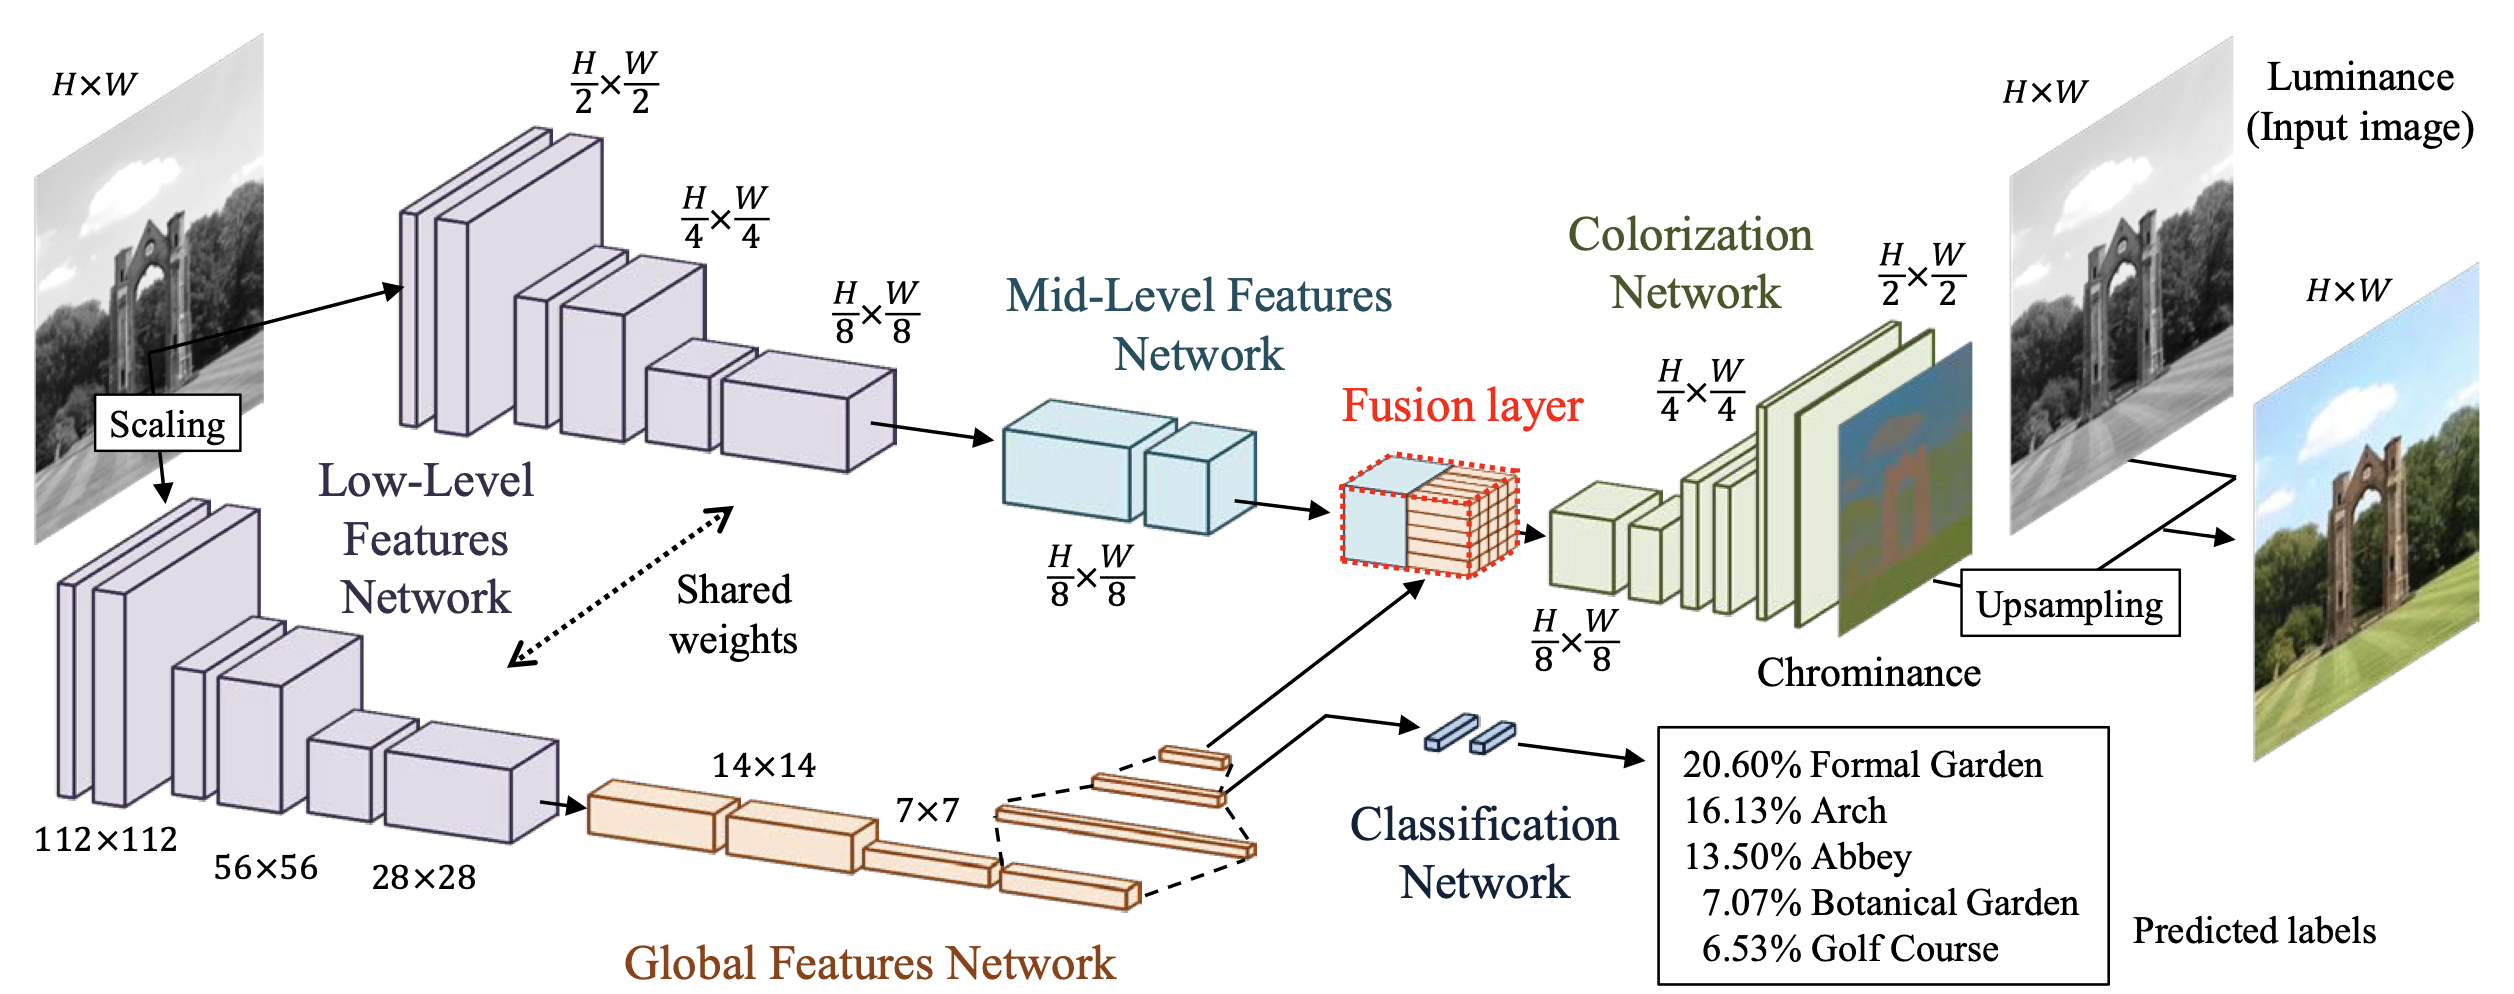
\includegraphics[width=\textwidth]{images/global-local-features.png}
%                     \caption{Let there be Color!: Joint End-to-end Learning of Global and Local Image Priors for Automatic Image Colorization with Simultaneous Classification 2016 \cite{iizuka2016let}.}
%                 \end{figure}
%             \end{frame}
%             \begin{frame}{Przegląd rozwiązań}
                
%                 \begin{figure}
%                     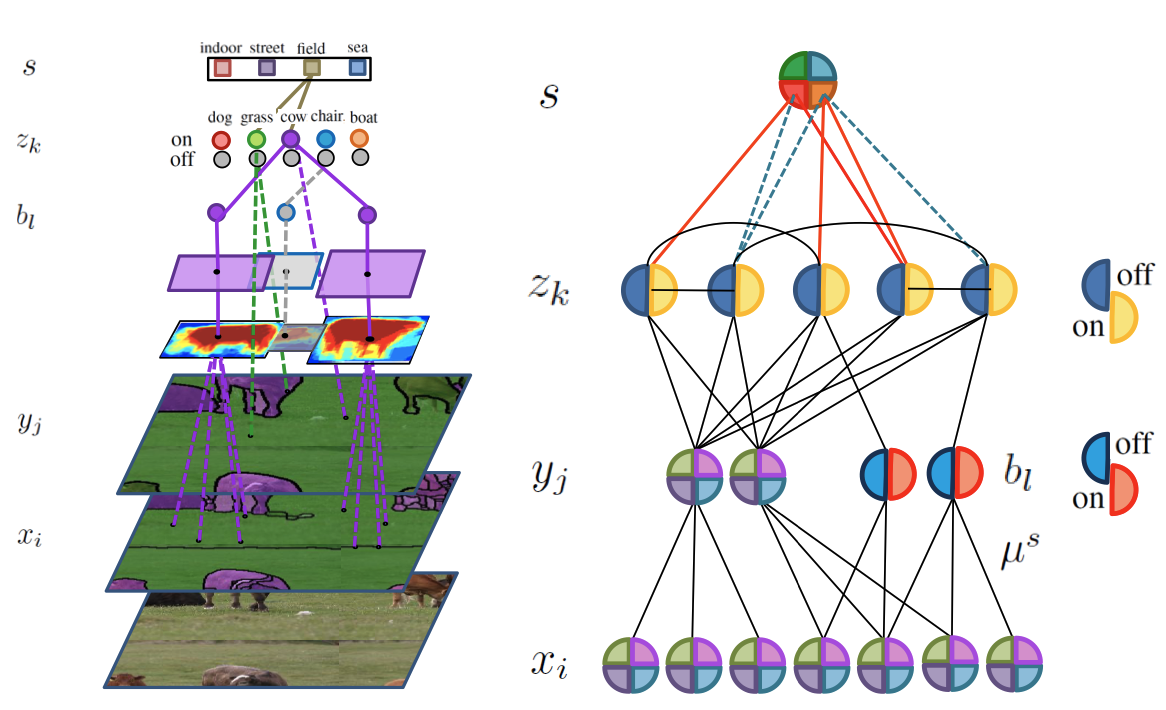
\includegraphics[width=\textwidth]{images/joint-segmentation-and-classification.png}
%                     \caption{Describing the Scene as a Whole: Joint Object Detection, Scene Classification and Semantic Segmentation 2012 \cite{yao2012describing}.}
%                 \end{figure}
%             \end{frame}
%             \section[Zaproponowane rozwiązanie]{Zaproponowane rozwiązanie}
%             % ########################################################################################################
%             \begin{frame}{Zaproponowane rozwiązanie}
                
%                 \begin{figure}
%                     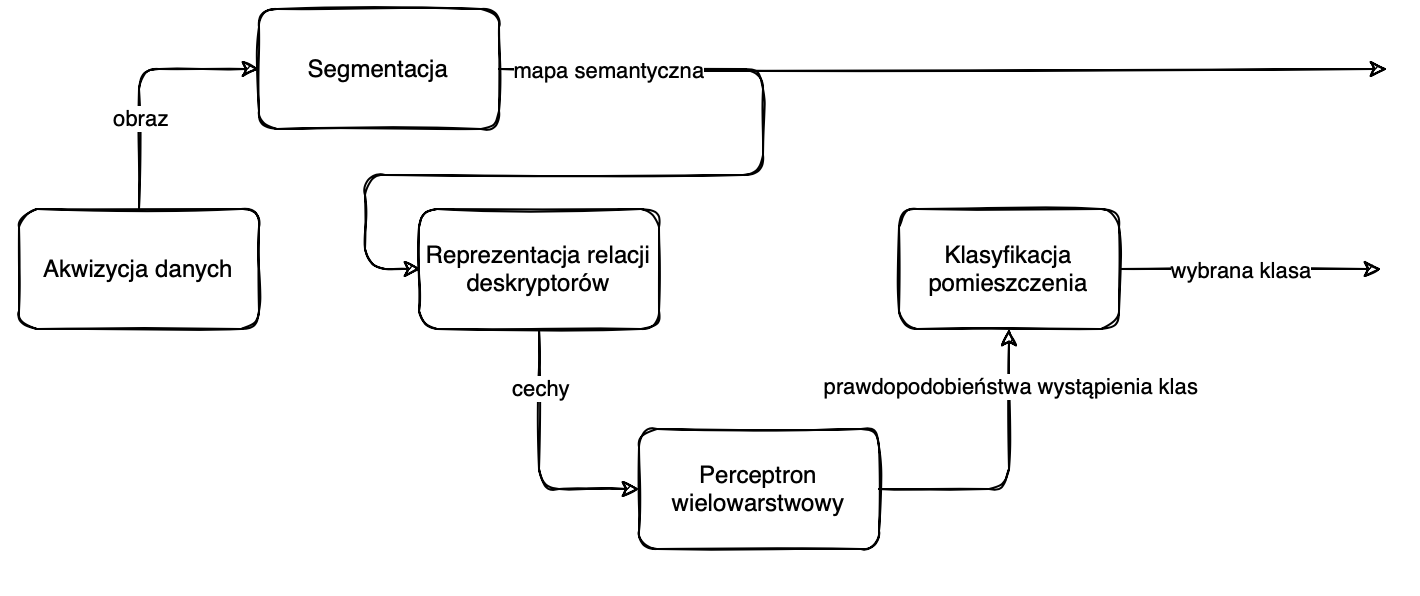
\includegraphics[width=\textwidth]{images/own-solution.png}
%                     \caption{Prototyp rozwiązania.}
%                 \end{figure}
                
% \end{frame}
% % \section{Plan prac}
% \begin{frame}{Plan prac}
%     \begin{table}[]

%         \begin{adjustbox}{width=\columnwidth,center}
%         \begin{tabular}{lllll}
%                                                                                 & październik & listopad & grudzień & styczeń \\
%         Przygotowanie zbioru danych                                                & x           &          &          &         \\ \hline
%         Model segmentacji                                                          & x           &          &          &         \\ \hline
%         Ekstrakcja cech                                                            & x           &          &          &         \\ \hline
%         Model klasyfikatora oraz trening                                           & x           &          &          &         \\ \hline
%         Ewaluacja rezultatów                                                       & x           & x        &          &         \\ \hline \hline
%         Implementacja Y-Netu                                                       &             & x        &          &         \\ \hline
%         Uczenie Y-Netu                                                             &             & x        &          &         \\ \hline
%         Ewaluacja rezultatów                                                       &             & x        & x        &         \\ \hline
%         Realizacja interesujących zagadnień\\ wynikających w czasie tworzenia pracy &             &          & x        & x      
%         \end{tabular}
%         \end{adjustbox}
%         \end{table}
% \end{frame}
% % ########################################################################################################
% \section[Podsumowanie]{Podsumowanie}
% % ########################################################################################################
% \begin{frame}{Podsumowanie}
%     Wkład w pracę skupia się wokół porównania różnych podejść do semantycznej analizy środowiska domowego \\


%     \underline{Wykonano:}

%     \begin{itemize}
%         \item Przegląd literatury i przygotowanie koncepcji systemu
%         \item Wybór i analiza zbioru danych
%         \item Zapoznanie z modelami segmentacji semantycznej
%     \end{itemize}
% \end{frame}



% %     \section[Założenia]{Założenia}
% % \begin{frame}{Założenia}

% %  \begin{itemize}
% %      \item Środowisko wewntątrz budynków, domowe
% %      \item Inferencja na robocie Tiago (MS Kinect)
% %  \end{itemize}
% % \end{frame}

% % % ########################################################################################################
% % \section[Motywacje]{Motywacje}
% % \begin{frame}{Motywacje}

% %  \begin{itemize}
% %      \item Nawigacja robota
% %      \begin{itemize}
% %          \item Wykrywanie przeszkód
% %          \item Zmiana zachowania pod wpływem znajdującego się pomieszczenia
% %      \end{itemize}
% %      \item Przewodnik dla osób niewidomych
% %      \item Predykcja afordancji
% %     %  \item Poprawa działania całokształtu poprzez głębsze zrozuemienie otoczenia
% %  \end{itemize}
% % \end{frame}
% % % ########################################################################################################
% % \section[Zbiór danych]{Zbiór danych}
% % \begin{frame}{Zbiór danych}
% %     Wymagania:
% %     \begin{itemize}
% %         \item MS Kinect
% %         \item Kategorie scen
% %         \item Maski obiektów
% %     \end{itemize}
    
% %    \end{frame}
% % % ########################################################################################################
% % \begin{frame}{Zbiór danych}
% %     \begin{table}[]
% %         \begin{adjustbox}{width=\columnwidth,center}
% %         \begin{tabular}{l|ccccccc}
% %         Nazwa    & \# Ilość & \# Klas obiektów & \# Klas scen & RGB-D     & Rozdzielczość & \# Czujników & Nieposprzątane \\ \hline \hline
% %         NYUv2    & 1 449    & 894              & 26           & \checkmark & 640 x 480     & 1            & \checkmark                   \\
% %         SUN RGBD & 10 335   & 800              & 47           & \checkmark & 640 x 480     & 4            & x                         
% %         \end{tabular}
% %         \end{adjustbox}
% %         \caption{Porówanie zbiorów danych \cite{song2015sun},\cite{silberman2012indoor}}
% %         \end{table}
% % \end{frame}
% %    % ########################################################################################################
% % \begin{frame}{Zbiór danych}
% %     \begin{figure}
% %         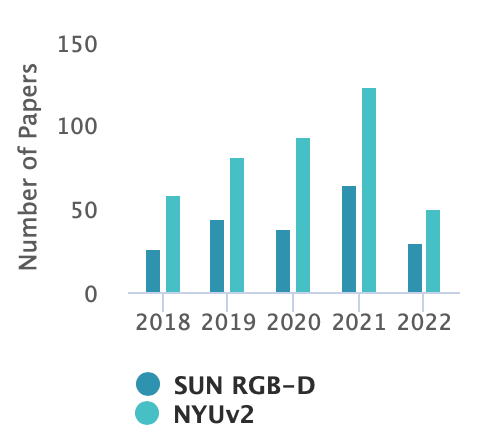
\includegraphics[height=0.7\textheight]{images/stats-dataset.png}
% %         \caption[]{Szacowana liczba cytowań w latach 2018-2022 \href{https://paperswithcode.com/dataset/sun-rgb-d}{[paperswithcode.com]}}
% %     \end{figure}
% % \end{frame}
% % ########################################################################################################
% % ########################################################################################################
% % ########################################################################################################
% % ########################################################################################################
% % ########################################################################################################







% % \begin{frame}[fragile]{Metropolis}
    
%     %   The \themename theme is a Beamer theme with minimal visual noise
%     %   inspired by the \href{https://github.com/hsrmbeamertheme/hsrmbeamertheme}{\textsc{hsrm} Beamer
%     %   Theme} by Benjamin Weiss.
    
%     %   Enable the theme by loading
    
%     %   \begin{verbatim}    \documentclass{beamer}
%         %     \usetheme{metropolis}\end{verbatim}
        
%         %   Note, that you have to have Mozilla's \emph{Fira Sans} font and XeTeX
%         %   installed to enjoy this wonderful typography.
%         % \end{frame}
%         % \begin{frame}[fragile]{Sections}
%             %   Sections group slides of the same topic
            
%             %   \begin{verbatim}    \section{Elements}\end{verbatim}
            
% %   for which \themename provides a nice progress indicator \ldots
  
% % \end{frame}

% % \section{Titleformats}

% % \begin{frame}{Metropolis titleformats}
% % 	\themename supports 4 different titleformats:
% % 	\begin{itemize}
% % 		\item Regular
% % 		\item \textsc{Smallcaps}
% % 		\item \textsc{allsmallcaps}
% % 		\item ALLCAPS
% % 	\end{itemize}
% % 	They can either be set at once for every title type or individually.
% % \end{frame}

% % \subsection{Tricks}

% % {
% %     \metroset{titleformat frame=smallcaps}
% % \begin{frame}{Small caps}
% % 	This frame uses the \texttt{smallcaps} titleformat.

% % 	\begin{alertblock}{Potential Problems}
% % 		Be aware, that not every font supports small caps. If for example you typeset your presentation with pdfTeX and the Computer Modern Sans Serif font, every text in smallcaps will be typeset with the Computer Modern Serif font instead.
% % 	\end{alertblock}
% % \end{frame}
% % }

% % {
% % \metroset{titleformat frame=allsmallcaps}
% % \begin{frame}{All small caps}
% % 	This frame uses the \texttt{allsmallcaps} titleformat.

% % 	\begin{alertblock}{Potential problems}
% % 		As this titleformat also uses smallcaps you face the same problems as with the \texttt{smallcaps} titleformat. Additionally this format can cause some other problems. Please refer to the documentation if you consider using it.

% % 		As a rule of thumb: Just use it for plaintext-only titles.
% % 	\end{alertblock}
% % \end{frame}
% % }

% % {
% % \metroset{titleformat frame=allcaps}
% % \begin{frame}{All caps}
% % 	This frame uses the \texttt{allcaps} titleformat.

% % 	\begin{alertblock}{Potential Problems}
% % 		This titleformat is not as problematic as the \texttt{allsmallcaps} format, but basically suffers from the same deficiencies. So please have a look at the documentation if you want to use it.
% % 	\end{alertblock}
% % \end{frame}
% % }

% % \section{Elements}

% % \begin{frame}[fragile]{Typography}
% %       \begin{verbatim}The theme provides sensible defaults to
% % \emph{emphasize} text, \alert{accent} parts
% % or show \textbf{bold} results.\end{verbatim}

% %   \begin{center}becomes\end{center}

% %   The theme provides sensible defaults to \emph{emphasize} text,
% %   \alert{accent} parts or show \textbf{bold} results.
% % \end{frame}

% % \begin{frame}{Font feature test}
% %   \begin{itemize}
% %     \item Regular
% %     \item \textit{Italic}
% %     \item \textsc{SmallCaps}
% %     \item \textbf{Bold}
% %     \item \textbf{\textit{Bold Italic}}
% %     \item \textbf{\textsc{Bold SmallCaps}}
% %     \item \texttt{Monospace}
% %     \item \texttt{\textit{Monospace Italic}}
% %     \item \texttt{\textbf{Monospace Bold}}
% %     \item \texttt{\textbf{\textit{Monospace Bold Italic}}}
% %   \end{itemize}
% % \end{frame}

% % \begin{frame}{Lists}
% %   \begin{columns}[T,onlytextwidth]
% %     \column{0.33\textwidth}
% %       Items
% %       \begin{itemize}
% %         \item Milk \item Eggs \item Potatos
% %       \end{itemize}

% %     \column{0.33\textwidth}
% %       Enumerations
% %       \begin{enumerate}
% %         \item First, \item Second and \item Last.
% %       \end{enumerate}

% %     \column{0.33\textwidth}
% %       Descriptions
% %       \begin{description}
% %         \item[PowerPoint] Meeh. \item[Beamer] Yeeeha.
% %       \end{description}
% %   \end{columns}
% % \end{frame}
% % \begin{frame}{Animation}
% %   \begin{itemize}[<+- | alert@+>]
% %     \item \alert<4>{This is\only<4>{ really} important}
% %     \item Now this
% %     \item And now this
% %   \end{itemize}
% % \end{frame}
% % \begin{frame}{Figures}
% %   \begin{figure}
% %     \newcounter{density}
% %     \setcounter{density}{20}
% %     \begin{tikzpicture}
% %       \def\couleur{alerted text.fg}
% %       \path[coordinate] (0,0)  coordinate(A)
% %                   ++( 90:5cm) coordinate(B)
% %                   ++(0:5cm) coordinate(C)
% %                   ++(-90:5cm) coordinate(D);
% %       \draw[fill=\couleur!\thedensity] (A) -- (B) -- (C) --(D) -- cycle;
% %       \foreach \x in {1,...,40}{%
% %           \pgfmathsetcounter{density}{\thedensity+20}
% %           \setcounter{density}{\thedensity}
% %           \path[coordinate] coordinate(X) at (A){};
% %           \path[coordinate] (A) -- (B) coordinate[pos=.10](A)
% %                               -- (C) coordinate[pos=.10](B)
% %                               -- (D) coordinate[pos=.10](C)
% %                               -- (X) coordinate[pos=.10](D);
% %           \draw[fill=\couleur!\thedensity] (A)--(B)--(C)-- (D) -- cycle;
% %       }
% %     \end{tikzpicture}
% %     \caption{Rotated square from
% %     \href{http://www.texample.net/tikz/examples/rotated-polygons/}{texample.net}.}
% %   \end{figure}
% % \end{frame}
% % \begin{frame}{Tables}
% %   \begin{table}
% %     \caption{Largest cities in the world (source: Wikipedia)}
% %     \begin{tabular}{lr}
% %       \toprule
% %       City & Population\\
% %       \midrule
% %       Mexico City & 20,116,842\\
% %       Shanghai & 19,210,000\\
% %       Peking & 15,796,450\\
% %       Istanbul & 14,160,467\\
% %       \bottomrule
% %     \end{tabular}
% %   \end{table}
% % \end{frame}
% % \begin{frame}{Blocks}
% %   Three different block environments are pre-defined and may be styled with an
% %   optional background color.

% %   \begin{columns}[T,onlytextwidth]
% %     \column{0.5\textwidth}
% %       \begin{block}{Default}
% %         Block content.
% %       \end{block}

% %       \begin{alertblock}{Alert}
% %         Block content.
% %       \end{alertblock}

% %       \begin{exampleblock}{Example}
% %         Block content.
% %       \end{exampleblock}

% %     \column{0.5\textwidth}

% %       \metroset{block=fill}

% %       \begin{block}{Default}
% %         Block content.
% %       \end{block}

% %       \begin{alertblock}{Alert}
% %         Block content.
% %       \end{alertblock}

% %       \begin{exampleblock}{Example}
% %         Block content.
% %       \end{exampleblock}

% %   \end{columns}
% % \end{frame}
% % % \begin{frame}{Math}
% % %   \begin{equation*}
% % %     e = \lim_{n\to \infty} \left(1 + \frac{1}{n}\right)^n
% % %   \end{equation*}
% % % \end{frame}
% % % \begin{frame}{Line plots}
% % %   \begin{figure}
% % %     \begin{tikzpicture}
% % %       \begin{axis}[
% % %         mlineplot,
% % %         width=0.9\textwidth,
% % %         height=6cm,
% % %       ]

% % %         \addplot {sin(deg(x))};
% % %         \addplot+[samples=100] {sin(deg(2*x))};

% % %       \end{axis}
% % %     \end{tikzpicture}
% % %   \end{figure}
% % % \end{frame}
% % % \begin{frame}{Bar charts}
% % %   \begin{figure}
% % %     \begin{tikzpicture}
% % %       \begin{axis}[
% % %         mbarplot,
% % %         xlabel={Foo},
% % %         ylabel={Bar},
% % %         width=0.9\textwidth,
% % %         height=6cm,
% % %       ]

% % %       \addplot plot coordinates {(1, 20) (2, 25) (3, 22.4) (4, 12.4)};
% % %       \addplot plot coordinates {(1, 18) (2, 24) (3, 23.5) (4, 13.2)};
% % %       \addplot plot coordinates {(1, 10) (2, 19) (3, 25) (4, 15.2)};

% % %       \legend{lorem, ipsum, dolor}

% % %       \end{axis}
% % %     \end{tikzpicture}
% % %   \end{figure}
% % % \end{frame}
% % \begin{frame}{Quotes}
% %   \begin{quote}
% %     Veni, Vidi, Vici
% %   \end{quote}
% % \end{frame}

% % {%
% % \setbeamertemplate{frame footer}{My custom footer}
% % \begin{frame}[fragile]{Frame footer}
% %     \themename defines a custom beamer template to add a text to the footer. It can be set via
% %     \begin{verbatim}\setbeamertemplate{frame footer}{My custom footer}\end{verbatim}
% % \end{frame}
% % }

% % \begin{frame}{References}
% %   Some references to showcase [allowframebreaks] 
% % \end{frame}

% % \section{Conclusion}

% % \begin{frame}{Summary}

% %   Get the source of this theme and the demo presentation from

% %   \begin{center}\url{github.com/matze/mtheme}\end{center}

% %   The theme \emph{itself} is licensed under a
% %   \href{http://creativecommons.org/licenses/by-sa/4.0/}{Creative Commons
% %   Attribution-ShareAlike 4.0 International License}.

% %   \begin{center}\ccbysa\end{center}

% % \end{frame}

% % {\setbeamercolor{palette primary}{fg=black, bg=yellow}
% % \begin{frame}[standout]
% %   Questions?
% % \end{frame}
% % }

% % \appendix

% % \begin{frame}[fragile]{Backup slides}
% %   Sometimes, it is useful to add slides at the end of your presentation to
% %   refer to during audience questions.

% %   The best way to do this is to include the \verb|appendixnumberbeamer|
% %   package in your preamble and call \verb|\appendix| before your backup slides.

% %   \themename will automatically turn off slide numbering and progress bars for
% %   slides in the appendix.
% % \end{frame}



